\documentclass[journal]{IEEEtran}

\usepackage[T1]{fontenc}

\usepackage{cite}
\usepackage{amsmath}
\interdisplaylinepenalty=2500
\usepackage{amssymb}
\usepackage{amsthm}
\usepackage{graphicx}
\usepackage{booktabs}
\usepackage{array}
\usepackage[caption=false,font=footnotesize,labelformat=simple,justification=centering]{subfig}
\usepackage{url}
\usepackage[hidelinks]{hyperref}

% Shared notation for every section (do not redefine elsewhere)
\newcommand{\BIG}{\mathsf{B}}                       % value of a passed pawn, B = 256
\newcommand{\pos}[1]{\texttt{#1}}                   % pawn list, e.g. \pos{W a2 c2 / B b7 d7}
\newcommand{\fen}[1]{\texttt{\small #1}}
\newcommand{\lab}[1]{\textsf{\footnotesize[#1]}}   % evidence label: \lab{P}, \lab{AI}, \lab{C2}, \lab{C1}, \lab{Conj}
\newcommand{\nim}[1]{\mathord{\star#1}}             % nimbers, as in the 2025 paper: \star, \nim{2}
\newcommand{\upsec}{\mathord{\uparrow^{2}}}         % up-second {0 | down star}
\newcommand{\tinyg}[1]{\operatorname{tiny}(#1)}
\newcommand{\game}[2]{\{\,#1 \mid #2\,\}}
\newcommand{\ggame}[2]{\{\,#1 \parallel #2\,\}}
\newcommand{\cyl}[1]{C_{#1}}                        % n-file cylinder
\newcommand{\flatb}[1]{F_{#1}}                      % n-file flat board
\newcommand{\repourl}{https://github.com/aritroBh/cylindrical-chess-cgt}


% The sections use the subcaption-style environment
%   \begin{subfigure}[pos]{width} ... \caption{...}\label{...} \end{subfigure}.
% IEEEtran's captions are kept by implementing it with subfig's \subfloat (caption=false), as the
% IEEEtran HOWTO recommends. A subfigure is labelled (a) and referenced as Fig. 3(a).
\renewcommand{\thesubfigure}{(\alph{subfigure})}
\makeatletter
\newsavebox{\sf@box}
\newcommand{\sf@setcap}[2][]{\gdef\sf@cap{#2}}
\newcommand{\sf@setlab}[1]{\gdef\sf@lab{#1}}
\newenvironment{subfigure}[2][c]{%
  \gdef\sf@cap{}\gdef\sf@lab{}%
  \begin{lrbox}{\sf@box}\begin{minipage}[#1]{#2}%
  \let\caption\sf@setcap\let\label\sf@setlab}%
  {\end{minipage}\end{lrbox}%
   \ifx\sf@lab\@empty\def\sf@labcmd{}\else\edef\sf@labcmd{\noexpand\label{\sf@lab}}\fi
   \ifx\sf@cap\@empty\subfloat[]{\usebox{\sf@box}\sf@labcmd}%
   \else\subfloat[\sf@cap\sf@labcmd]{\usebox{\sf@box}}\fi}
\makeatother

% One counter for all numbered statements, through the whole paper, in IEEE style:
% an indented italic head ending in a colon ("Theorem 2 (Cut lemma; [P]):").
\newtheoremstyle{ieeeplain}{3pt}{3pt}{\itshape}{\parindent}{\itshape}{:}{0.5em}{}
\newtheoremstyle{ieeedef}{3pt}{3pt}{\normalfont}{\parindent}{\itshape}{:}{0.5em}{}
\theoremstyle{ieeeplain}
\newtheorem{theorem}{Theorem}
\newtheorem{lemma}[theorem]{Lemma}
\newtheorem{proposition}[theorem]{Proposition}
\newtheorem{corollary}[theorem]{Corollary}
\newtheorem{conjecture}[theorem]{Conjecture}
\theoremstyle{ieeedef}
\newtheorem{definition}[theorem]{Definition}
\newtheorem{remark}[theorem]{Remark}
% Proofs use IEEEtran's proof layout; \begin{proof}[Proof sketch] prints "Proof sketch:".
\renewenvironment{proof}[1][Proof]{\begin{IEEEproof}[#1]}{\end{IEEEproof}}

\hyphenation{tr\'e-bu-chet tr\'e-bu-chets table-base table-bases}

\begin{document}

\title{Chess Endgames on a Cylindrical Chessboard: Exact Combinatorial Game Values, Real-Chess Checks,
and Tablebases}

\author{Aritro~Bhattacharjee%
\thanks{A.~Bhattacharjee, e-mail: aritro.sonu@gmail.com.}}

\markboth{Bhattacharjee: Chess Endgames on a Cylindrical Chessboard}%
{Bhattacharjee: Chess Endgames on a Cylindrical Chessboard}

\maketitle

\begin{abstract}
Cylinder chess joins the a-file to the h-file, so the board has no edges or corners. We study its
king-and-pawn endgames with combinatorial game theory, following Elkies: a passed pawn counts as a win, and a
mutual zugzwang of the kings counts as zero. We first repair this model. We replace the usual passed-pawn test,
which ignores en passant, with one that respects it, and we give conditions under which frozen kings are
exact. Under the new test, an exhaustive census of small positions finds no nimber above star with six pawns or
fewer, but star two appears with seven pawns, in two positions confirmed by three independent programs. We also
find one-eighth, up-second star and Tiny 1, and test the model against real chess with
endgame tablebases. For the one-eighth position, a queen-promotion search leaves one undecided end
position, with black to move, on which its value depends. Four-man tablebases on the cylinder and the torus show
that king and rook can no longer force mate. We correct the earlier analysis of Dawson's chess on the cylinder
and prove that the full ring is a first-player win exactly when the strip three files shorter has Grundy value
zero.
\end{abstract}

\begin{IEEEkeywords}
Chess, combinatorial game theory, endgame tablebases, game solving, nimbers.
\end{IEEEkeywords}


\section{Introduction}\label{sec:intro}

\IEEEPARstart{C}{ylinder} chess is ordinary chess played on a board whose a-file and h-file are joined
\cite{Pritchard}. A white pawn on h4 can capture on a5, a king on a1 can step to h2, and every file is like every
other: the board has no edges and no corners (Fig.~\ref{fig:cover}). In this paper we use combinatorial game
theory (CGT) to study king-and-pawn endgames on this board.

Under normal play, the player who cannot move loses. CGT gives each position of such a game a value, and the
value of a sum of independent games is the sum of their values \cite{ONAG,WinningWays,Siegel2013}. Chess is not
such a game: it can be drawn, and the kings can walk from one part of the board to another. Even so, Elkies
\cite{Elkies1996} showed that many pawn endgames split into local fights whose values are numbers, star,
infinitesimals such as up, and hot switches. Two conventions make this work:
\begin{itemize}
\item a side that gets a passed pawn wins, so a passed pawn is worth a large number $\pm\BIG$;
\item the kings stand in a mutual zugzwang, the \emph{tr\'ebuchet}, which counts as $0$.
\end{itemize}
Wu, Y\"u and Landry \cite{WuYuLandry2020} worked through these ideas position by position, and we follow
their format.

The cylinder changes this picture in three ways. There are no rook pawns, and a position can be shifted
sideways by any number of files without changing its value. A position with a pawn on every file, a
\emph{ring}, has no edge at which to cut it. And the corners that decide mates and fortresses on the ordinary
board are gone.

\begin{figure}[!t]
\centering
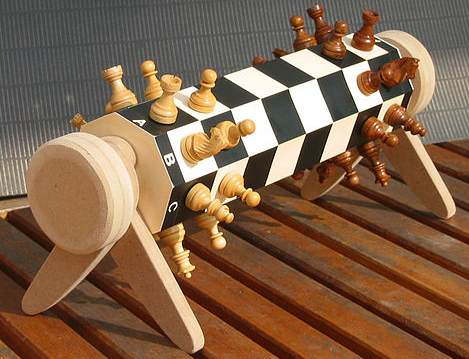
\includegraphics[width=0.6\columnwidth]{figures/CoverPic.png}
\caption{Cylindrical chessboard with all pieces on their starting squares; files a and h are adjacent.
Photograph by S.~Clair, Wikimedia Commons, CC BY-SA 3.0~\cite{CoverImage}.}
\label{fig:cover}
\end{figure}

The simplest nimber after $\star$ is $\nim{2}=\game{0,\star}{0,\star}$, a game in which either player may move
to $0$ or to $\star$. Elkies later built higher nimbers in pawn endgames on large boards by
adapting Dawson's pawn game \cite{Elkies2002,Dawson1935}, and Drummond-Cole gave positions of value $\nim{2}$
in generalized Domineering and in chess \cite{DrummondCole2005}. We ask whether $\nim{2}$ occurs in a
king-and-pawn endgame on a board with eight ranks, the \emph{$\nim{2}$ question}, and, where the model says
$\nim{2}$, whether real chess agrees.

This paper extends an unpublished 2025 study\bytheauthor~\cite{Bhattacharjee2025}, which built the basic
values on the cylinder by hand; here every position is checked by computer, the errors of that study are
corrected where they occur, and the analysis is carried on to the questions above. Because so much of the work
is computational, each theorem and headline number carries a label: \lab{P} proved, \lab{C2} checked by two
independent programs, \lab{C1} computed by one program, and \lab{Conj} a conjecture. Our contributions are as
follows.
\begin{itemize}
\item \emph{An exact model} (Sections~\ref{sec:rules} and~\ref{sec:sums}). The textbook passed-pawn test ignores
  en passant; we replace it, prove a cut lemma and a sum-safety theorem \lab{P}, and show that the earlier
  sum-safety test fails \lab{C2}.
\item \emph{Kings} (Section~\ref{sec:kings}). We give conditions (V1)--(V4) under which a frozen tr\'ebuchet
  gives the true chess result \lab{P}; on small boards the convention, with the textbook test, fails for 159 of
  500 components \lab{C1}.
\item \emph{Small values} (Sections~\ref{sec:atlas} and~\ref{sec:targets}). Every value that only the cylinder
  can make comes from a ring \lab{P}, and $1/8$, $\upsec\star$ and Tiny~1 occur in legal 10-man positions
  \lab{C2}.
\item \emph{The $\nim{2}$ question} (Section~\ref{sec:star2}). Under the new test no $\nim{2}$ exists with six
  pawns or fewer on boards of width at most four, but two exist with seven \lab{C2}.
\item \emph{Real chess} (Section~\ref{sec:real}). In the e.p.-aware pawn tree, the real-chess value of the
  textbook candidate is never $\nim{2}$, however draws are treated, and the $1/8$ hinges on one end position
  that a queen-promotion search leaves open \lab{C1}.
\item \emph{Tablebases} (Section~\ref{sec:tb}). On the cylinder king and rook win only 2.80\% of positions
  \lab{C2}.
\item \emph{Dawson's chess} (Section~\ref{sec:dawson}). The $3\times n$ cylinder is a first-player win if and
  only if the $3\times(n-3)$ strip has Grundy value $0$ \lab{P}.
\item \emph{Engines} (Section~\ref{sec:engines}). Stockfish is weakest on infinitesimals at low depth \lab{C1}.
\end{itemize}

Sections~\ref{sec:rules}--\ref{sec:basic} set up the rules and the basic values,
Sections~\ref{sec:kings}--\ref{sec:sums} add kings and sums, Sections~\ref{sec:atlas}--\ref{sec:real} search for
small values and test them against real chess, and Sections~\ref{sec:tb}--\ref{sec:engines} turn to tablebases,
Dawson's chess and engines. Section~\ref{sec:verify} explains how each result was checked, and
Section~\ref{sec:conclusion} lists open problems.

\section{Rules, Values and Conventions}\label{sec:rules}

\subsection{The Board and the Moves}
We play ordinary chess, but on a different board. As usual the files are a, b, \dots, h and the ranks, from
bottom to top, are 1, \dots, 8. The cylindrical board is the $8\times 8$ board with the a-file joined to the
h-file. Only the files wrap: ranks 1 and 8 are still edges, and pawns still promote. Every piece may cross the
seam between the h- and a-files. Thus a white pawn on h4 can capture a black pawn on a5, a knight on b2 can move
to h3, and a knight on h1 gains the squares a3 and b2. A king on h1 gains a1 and a2, so a checkmate on the
ordinary board need not be a checkmate on the cylinder. A rook, bishop or queen may slide across the seam, but
it stops before its ray returns to its own square, so it cannot go round a rank as a null move. En passant
(e.p.) is allowed, including across the seam. All files are now equivalent, and there are no edge pawns. We
write $\cyl{n}$ for the cylinder with $n$ files and $\flatb{n}$ for the ordinary (flat) board with $n$ files,
both with eight ranks.

\subsection{Normal Play and the Passed-Pawn Convention}
Chess is not a normal-play game: it can be drawn, and the winner is decided by checkmate, not by who moves
last \cite{WinningWays}. Following Elkies \cite{Elkies1996}, we change it just enough to fit the theory.
\begin{itemize}
\item In pawn-only positions, a player who has no move loses. There are no null moves: a player must move on
  every turn.
\item A position in which exactly one side has a passed pawn is decided. It is worth $+\BIG$ if white has the
  passed pawn and $-\BIG$ if black has it, where $\BIG$ is larger than any count of spare moves that can arise
  (our programs use $\BIG=256$).
\item Kings are added as a group in mutual zugzwang, the tr\'ebuchet, which counts as the zero game: whoever
  has to move a king there loses a pawn, and then the game. Section~\ref{sec:kings} asks when this is exact.
\end{itemize}
So a standard win is a checkmate, while a normal-play win is a passed pawn, or an opponent with no move.

A single move, usually a capture, can give both sides a passed pawn at once. Such a promotion race needs a
rule:
\begin{itemize}
\item \emph{count}: the side that did not make the move goes first in the race; whoever needs fewer moves to
  promote wins, and a tie goes to the side that goes first;
\item \emph{mover}: the side that made the move wins;
\item \emph{opponent}: the other side wins.
\end{itemize}
None of the three is exact chess, since a new queen may give check or stop the other pawn.

\subsection{En Passant and the Passed-Pawn Test}
The convention needs a test for ``passed''. The textbook test calls a pawn passed if no enemy pawn stands ahead
of it on its own file or on a neighboring file (on the cylinder, the a- and h-files are neighbors). En passant
breaks this test. In Fig.~\ref{fig:ep_test}, white plays a2--a4. No black pawn now stands ahead of the a-pawn on
the a- or b-file, so the textbook test calls it passed. But black can answer b4$\times$a3 en passant, and the
``passed'' pawn is gone. So we use a stricter test.

\begin{figure}[!t]
\centering
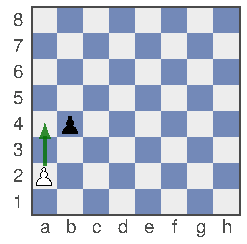
\includegraphics[width=0.42\columnwidth]{figures/ep_test.pdf}
\caption{White a2 against black b4 (ordinary board), value $0$. After a2--a4 (arrow) no black pawn stands ahead
of the a-pawn, but black may capture it en passant, b4$\times$a3, so under Definition~\ref{def:epaware} it is
not passed.}
\label{fig:ep_test}
\end{figure}

\begin{definition}[E.p.-aware passed pawn]\label{def:epaware}
A pawn is \emph{passed} if no enemy pawn stands ahead of it on its own file or a neighboring file,
\emph{and} it cannot be captured en passant on the opponent's next move, that is, it has not just made a
double step to a square beside an enemy pawn.
\end{definition}

With one more white pawn the difference decides the game. In \pos{W a2 b3 / B b4}, black has no move. The
textbook test says that white wins at once with a2--a4. Under Definition~\ref{def:epaware}, every white move
lets black capture on a3, directly after a2--a3 and en passant after a2--a4, and win the promotion race that
follows under the count rule. So the second player wins, and the value is $0$. Across the flat census of
Section~\ref{sec:atlas}, every position with at most six pawns on boards of width at most four, the stricter
test changes $21{,}441$ of the $231{,}071$ values, $4{,}068$ of them in outcome \lab{C1}.

The three race rules and three treatments of en passant (the textbook test, the e.p.-aware test, and e.p.\
off) give nine \emph{settings}. Our default setting is the count rule with the e.p.-aware test; every value
uses it unless we say otherwise.

\subsection{Components and the Cut Lemma}
A pawn changes file only when it captures, and it can only capture onto a file where an enemy pawn already
stands (en passant included). So an empty file stays empty forever, and the pawns on either side of it never
interact. Each block of neighboring occupied files is therefore a game of its own, a \emph{component}, and a
position is the sum of its components. On the ordinary board the components are blocks of adjacent files. On
the cylinder they are arcs, or one \emph{ring} that uses every file.

\begin{theorem}[Cut lemma; \lab{P}, \lab{C2}]\label{thm:cut}
A pawn position on $\cyl{n}$ with at least one empty file has the same value as the position on
$\flatb{n-1}$ obtained by cutting the cylinder open along that file.
\end{theorem}

\begin{proof}
No pawn can ever move onto the empty file, so no move ever crosses it. Cutting the board there changes no legal
move, no en passant right and no passed-pawn test, because the files beside the cut lose only a neighbor that
stays empty forever.
\end{proof}

Hence values that only a cylinder can make must come from rings (Section~\ref{sec:atlas}).
Section~\ref{sec:sums-hss} gives the condition under which a sum of components still names the right winner.

\subsection{Notation}
We write $G=\game{G^L}{G^R}$ when white (Left) can move to the positions $G^L$ and black (Right) to the
positions $G^R$, and $G+H$ for the sum in which the player to move chooses one component
\cite{WinningWays,ONAG,Siegel2013}. Every finite game has a unique \emph{canonical form}, obtained by deleting
dominated options and bypassing reversible ones, and $G=H$ exactly when $G-H$ is a second-player win. The
\emph{outcome class} of $G$ is $\mathcal{L}$ if white wins whoever starts, $\mathcal{R}$ if black does,
$\mathcal{N}$ if the first player wins and $\mathcal{P}$ if the second player wins. Our values are
\emph{numbers} (integers and dyadic fractions such as $1/2=\game{0}{1}$), \emph{nimbers}
($\star=\game{0}{0}$ and $\nim{2}=\game{0,\star}{0,\star}$), \emph{ups} (${\uparrow}=\game{0}{\star}$,
${\Uparrow}={\uparrow}+{\uparrow}$ and ${\downarrow}=-{\uparrow}$), \emph{up-second} $\upsec=\game{0}{{\downarrow}\star}$,
\emph{tinies} $\tinyg{x}=\ggame{0}{0\mid -x}$ and \emph{switches} $\pm x=\game{x}{-x}$, with
$a\pm x=\game{a+x}{a-x}$. A sum of such values is written without the plus sign, as in
${\Uparrow}\star={\Uparrow}+\star$. The \emph{birthday} of a game is the height of its canonical game tree, so
$\nim{k}$ has birthday $k$. Each game has a \emph{mean} and a \emph{temperature}, read from its thermograph
\cite{WinningWays}. The temperature measures how much the player to move gains by moving first; $\pm x$ has
temperature $x$. Infinitesimals such as $\star$, ${\uparrow}$ and $\tinyg{1}$ have mean and temperature $0$, yet
they still decide sums. The \emph{left} and \emph{right stops} of $G$ are the numbers reached when white or black
moves first and both sides play until a number appears; both stops of $0$ and of $\nim{2}$ are $0$.

\section{Basic Positions on the Cylinder}\label{sec:basic}

\begin{figure*}[!t]
\centering
\begin{subfigure}[t]{0.235\textwidth}\centering
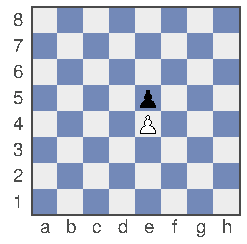
\includegraphics[width=\linewidth]{figures/zero.pdf}
\caption{\pos{W e4 / B e5}: $0$}
\end{subfigure}\hfill
\begin{subfigure}[t]{0.235\textwidth}\centering
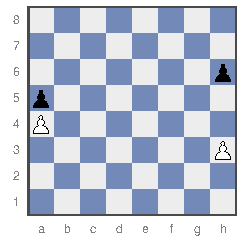
\includegraphics[width=\linewidth]{figures/zero_seam.pdf}
\caption{\pos{W a4 h3 / B a5 h6}: $0$}
\end{subfigure}\hfill
\begin{subfigure}[t]{0.235\textwidth}\centering
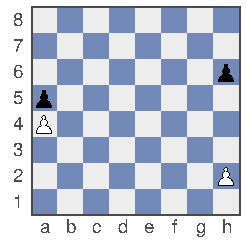
\includegraphics[width=\linewidth]{figures/one.pdf}
\caption{\pos{W a4 h2 / B a5 h6}: $1$}
\end{subfigure}\hfill
\begin{subfigure}[t]{0.235\textwidth}\centering
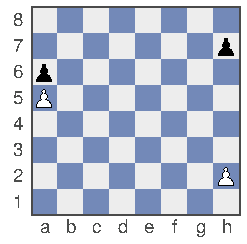
\includegraphics[width=\linewidth]{figures/two.pdf}
\caption{\pos{W a5 h2 / B a6 h7}: $2$}
\end{subfigure}

\medskip
\begin{subfigure}[t]{0.235\textwidth}\centering
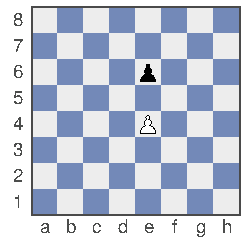
\includegraphics[width=\linewidth]{figures/star.pdf}
\caption{\pos{W e4 / B e6}: $\star$}
\end{subfigure}\hfill
\begin{subfigure}[t]{0.235\textwidth}\centering
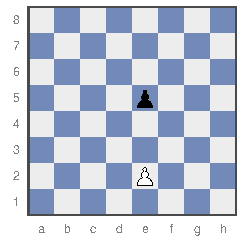
\includegraphics[width=\linewidth]{figures/up.pdf}
\caption{\pos{W e2 / B e5}: ${\uparrow}$}
\end{subfigure}\hfill
\begin{subfigure}[t]{0.235\textwidth}\centering
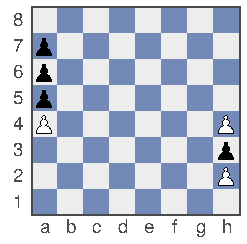
\includegraphics[width=\linewidth]{figures/tiny1_2025.pdf}
\caption{\pos{W a4 h2 h4 / B a5 a6 a7 h3}: $\tinyg{1}$}
\end{subfigure}\hfill
\begin{subfigure}[t]{0.235\textwidth}\centering
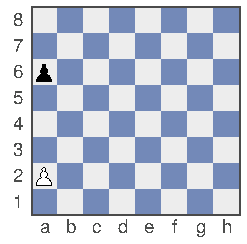
\includegraphics[width=\linewidth]{figures/elkies_dup.pdf}
\caption{\pos{W a2 / B a6}: ${\Uparrow}\star$}
\end{subfigure}
\caption{Basic pawn games. Boards (a)--(g) are cylinders (files a and h adjacent); (h) is drawn on the ordinary
board and has the same value on the cylinder. Each value holds under all three race rules, under both
passed-pawn tests, and with e.p.\ on or off, except (d), which is $2$ only with e.p.\ on and ${\Uparrow}\star$
with e.p.\ off.}
\label{fig:basic}
\end{figure*}

We first build the basic games $0$, $1$, $2$, $\star$, ${\uparrow}$ and Tiny 1 with pawns alone
(Fig.~\ref{fig:basic}); kings join in Section~\ref{sec:kings}. A full discussion of these simple games can be found in \cite{WinningWays}, and their
ordinary-board versions in \cite{Elkies1996,WuYuLandry2020}. Each board in Fig.~\ref{fig:basic} leaves a
file empty, so by Theorem~\ref{thm:cut} it is also a position on an ordinary board: these are Elkies' values,
and the cylinder lets four of them be built across the seam. Values that only a cylinder can make need a pawn on every file
(Section~\ref{sec:atlas}). One remark keeps the walk-throughs short. A move that lets the opponent reply with a
passed pawn, or with anything as bad, is reversible and drops out of the canonical form
\cite{WinningWays}: having only losing moves is the same as having no moves at all \cite{WuYuLandry2020}.

\subsection{The Zero Game}
Let's begin with the zero game, a game in which neither player can move: $0=\game{}{}$. Under normal play it is
a second-player win. In Fig.~\ref{fig:basic}(a) the two pawns in the center are stuck, so neither side has a
move, and the value is $0$.

Fig.~\ref{fig:basic}(b) is a zero game that uses the seam. If white goes first, it must play h3--h4, and the
black pawn on a5 captures it across the seam, a5$\times$h4, leaving a passed pawn. If black goes first, h6--h5
is met by a4$\times$h5 in the same way. Whoever moves first loses, so this is again $0$. As in
\cite{WuYuLandry2020}, many zero games are symmetric like this one.

\subsection{The Games \texorpdfstring{$1$}{1} and \texorpdfstring{$2$}{2}}
In Fig.~\ref{fig:basic}(c) the deadlocked pawns on a4 and a5 stay, but the white h-pawn starts one square
further back. White can play h2--h3, which leaves the zero game of Fig.~\ref{fig:basic}(b); the double step
h2--h4 only loses the pawn to a5$\times$h4. Black has one move, h6--h5, and a4$\times$h5 gives white a passed
pawn. Thus $G=\game{0}{}=1$, the one game.

In Fig.~\ref{fig:basic}(d) the a-pawns stand one rank higher, and the white h-pawn has two squares to cross.
White can play h2--h4, which leaves the zero game (b) moved up one rank, or h2--h3, which leaves the one game
(c) moved up one rank. Black has only losing moves: h7--h6 is met by a5$\times$h6, and the double step h7--h5 by
a5$\times$h6 en passant across the seam. Thus $G=\game{0,1}{}=2$, the two game. This value needs en passant:
with e.p.\ off, h7--h5 is safe and the value falls to ${\Uparrow}\star$. To get $-1$ or $-2$, switch the black and
white pawns and turn the board through $180^\circ$ \cite{WuYuLandry2020}.

\subsection{The Infinitesimals \texorpdfstring{$\star$, ${\uparrow}$}{Star, Up} and Tiny 1}
The first infinitesimal is star, in which both white and black can move to the zero game:
$\star=\game{0}{0}$. In Fig.~\ref{fig:basic}(e), e4--e5 and e6--e5 each lock the file, so $G=\star$, a
first-player win.

The formal definition of up is ${\uparrow}=\game{0}{\star}$. In Fig.~\ref{fig:basic}(f), white can play e2--e3,
which leaves star, or e2--e4, which locks the file and leaves $0$. Black can only play e5--e4, which leaves
star. Thus $G=\game{0,\star}{\star}$. Star is a reversible move for white: black answers e2--e3 with e5--e4 and
reaches $0$, and since white wins $G$ when black starts ($G\ge 0$), this reply is at least as good for black as
the position before white's move. So $G=\game{0}{\star}={\uparrow}$. Up is positive, so white wins whoever
starts, yet it is smaller than every positive number. Switching the colors as above gives ${\downarrow}$.

Tiny 1 is defined as $\tinyg{1}=\ggame{0}{0\mid -1}$. In Fig.~\ref{fig:basic}(g), white can take the black
pawn across the seam, h4$\times$a5, which leaves every pawn blocked: $0$. White can also advance h4--h5, but
black answers a6$\times$h5 and wins, so this move drops out. Black can only take white's pawn, a5$\times$h4.
From there white can lock the a-file with a4--a5, leaving $0$, while black can play a6--a5 and keep the spare
move a7--a6, leaving $-1$. So black's capture leads to $\game{0}{-1}=-\tfrac12\pm\tfrac12$, and
$G=\ggame{0}{0\mid -1}=\tinyg{1}$, a positive infinitesimal.

A single file can hold more than one might expect. In Fig.~\ref{fig:basic}(h), white can play a2--a3, leaving
$0$ (each side's move from there leaves star), or a2--a4, leaving $\star$. Black can only play a6--a5, which
leaves the up position of Fig.~\ref{fig:basic}(f) on the a-file. So $G=\game{0,\star}{{\uparrow}}$. Just as in
(f), star is reversible for white, so $G=\game{0}{{\uparrow}}={\Uparrow}\star$, ``double-up star'', one of Elkies'
examples \cite{Elkies1996}.

\section{Kings: the Tr\'ebuchet and When It Is Exact}\label{sec:kings}

So far a player with no pawn move simply lost. In chess that player would be stalemated, which is a draw.
Following Elkies~\cite{Elkies1996}, we therefore add the kings in a \emph{tr\'ebuchet}, a king group in mutual
zugzwang that the convention reads as the zero game. In this section we put the kings back on the board and
ask when that reading gives the true chess result. For this we use an exact king-and-pawn solver that plays
real chess: kings, pawns, en passant, all four promotions, stalemate, and no fifty-move rule. An independent
reference solver, written from the rules alone, agrees with it on all $1{,}418{,}480$ positions of its test runs
\lab{C2}, and on the ordinary board we also compare it with the Lichess tablebase~\cite{LichessTB}.

\subsection{Two Tr\'ebuchets}

In Fig.~\ref{fig:trebuchet_2025} the pawns on a4 and a5 block each other, so only the kings can move. The white
king on h5 guards a4 across the seam, and the black king on b4 guards a5. If white (Left) moves first, every king
move gives up a4: the only free square next to a4 that the king can reach, h4, is attacked by the a5 pawn
across the seam. In the same way black (Right), moving first, loses a5, since b5 is attacked by the a4 pawn.
Whichever player goes first will lose a pawn, allowing the other side's pawn to advance and promote. Thus this
position is a zero game. On an ordinary board the king on h5 would not touch a4, so the zugzwang exists only
because of the seam. With the kings played out it is a real mutual zugzwang: with white to move black wins, and
with black to move white wins \lab{C2}.

Fig.~\ref{fig:trebuchet} shows the same idea on files f to h of the ordinary board: the white king's only free
square next to g4, f4, is attacked by the g5 pawn, and the black king's only one next to g5, h5, by the g4 pawn.
The Lichess tablebase confirms that it is a real mutual zugzwang \lab{C2}. This is the king group we place
beside every ordinary-board pawn position in this paper.

\begin{figure}[!t]
\centering
\begin{subfigure}{0.48\columnwidth}
\centering
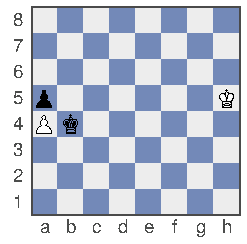
\includegraphics[width=\linewidth]{figures/trebuchet_2025.pdf}
\caption{Kh5, Pa4 / Kb4, Pa5 (cylinder: files a and h adjacent).}
\label{fig:trebuchet_2025}
\end{subfigure}\hfill
\begin{subfigure}{0.48\columnwidth}
\centering
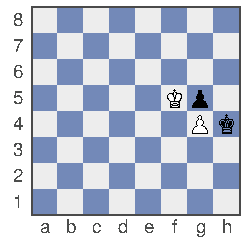
\includegraphics[width=\linewidth]{figures/trebuchet.pdf}
\caption{Kf5, Pg4 / Kh4, Pg5 (ordinary board).}
\label{fig:trebuchet}
\end{subfigure}

\medskip
\begin{subfigure}{0.48\columnwidth}
\centering
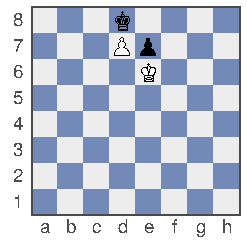
\includegraphics[width=\linewidth]{figures/kinggroup72.pdf}
\caption{Ke6, Pd7 / Kd8, Pe7 (cylinder; the seam plays no part).}
\label{fig:kinggroup72}
\end{subfigure}
\caption{King groups that the convention reads as $0$. (a) and (b) are tr\'ebuchets and real mutual
zugzwangs. (c) is the king group of Puzzle~2: with black to move white wins, but with white to move it is a
draw.}
\label{fig:kings}
\end{figure}

\subsection{When Is the Frozen Tr\'ebuchet Exact?}

A \emph{king group} $Z$ is the two kings and some pawns on a block of files, with no pawns on the neighboring
files (the \emph{buffer}). Pawns change file only by capturing, so the buffer stays empty and no pawn crosses
it. A \emph{decisive event} is a move that creates a passed pawn, or a move inside $Z$.

\begin{theorem}[Validity of the convention; \lab{P}]\label{thm:validity}
Let a king-and-pawn position consist of pawn components and a king group $Z$ with its buffer. Suppose that at
every position before the first decisive event:
\begin{enumerate}
\item[(V1)] the kings never interact with the components: the legal chess moves are exactly the moves of the
  model, en passant included, nobody is in check, and the side to move has a legal move;
\item[(V2)] every decisive event really wins: the side that gets a passed pawn wins the game;
\item[(V3)] every move inside $Z$, by either side, is decisively punished.
\end{enumerate}
Then, with either side to move, the chess result is the normal-play outcome of the pawn components alone, and
there are no draws. If moreover
\begin{enumerate}
\item[(V4)] no two components ever carry passed-pawn threats of opposite sign, and $\BIG$ exceeds every tempo
  count,
\end{enumerate}
then it is also the outcome class of the $\pm\BIG$ value of the components.
\end{theorem}

\begin{proof}[Proof sketch]
By (V3) every move in $Z$ loses, so the model is the normal-play sum of the components, a short game without
draws. Its winner $\sigma$ follows a winning strategy and never moves in $Z$. By (V1) every legal move of the
loser is a move of the model, and the loser always has one, so play ends at a decisive event in $\sigma$'s
favour: a passed pawn for $\sigma$, or a forced move of the loser in $Z$. By (V2) and (V3), $\sigma$ wins the
chess game. Under (V4), the argument of Theorem~\ref{thm:hss} gives the same outcome class for $\pm\BIG$.
\end{proof}

The proof shows what the tr\'ebuchet is really for: it turns stalemate into a loss, by always offering the side
without a pawn move a legal, losing move. Each condition can fail: a king walks over to the pawns (V1), a passed
pawn loses its race (V2), white's king moves in Fig.~\ref{fig:kinggroup72} are not punished (V3), and a $+\BIG$
in one component cancels a $-\BIG$ in another (V4; Section~\ref{sec:sums-hss}).

Condition (V3) depends on the other components, but it has a local certificate with horizon $T$: after the
punishing capture, and with all other pawns removed, the punisher promotes within $T$ moves even if the
defender may pass at any time; the defender cannot promote anywhere within $T$ moves; and the defender is never
stalemated in that window. The certificate implies (V3) for that move \lab{P}.

\begin{proposition}[\lab{P}]\label{prop:horizon1}
A punishment with a local certificate of horizon $T=1$ is decisive in every context without a passed pawn.
\end{proposition}

\begin{proof}
A pawn that could promote in one move stands on its seventh rank with no enemy pawn ahead, so it is already
passed.
\end{proof}

\begin{conjecture}[\lab{Conj}]\label{conj:horizon2}
For every $T\ge2$ there is a context without a passed pawn in which the certificate of horizon $T$ fails.
\end{conjecture}

In a real tr\'ebuchet the punisher, after winning the pawn, still needs $T\approx5$--$7$ moves to promote, so
the certificate does not cover every context: we trust its zero only beside slow or locked components.

\subsection{Spare King Moves Are Loopy}

A king that can step back and forth forever without loss is not $0$. It gives its side an unlimited supply of
waiting moves, a loopy game~\cite{WinningWays,Siegel2013}: $\textsf{on}=\game{\textsf{on}}{}$ if only white can
wait, $\textsf{off}=\game{}{\textsf{off}}$ if only black can, and $\textsf{dud}$ if both can. Since
$\textsf{on}$ exceeds every number, $\BIG$ included, any sum plus $\textsf{on}$ is a white win, even when black
has a forced passed pawn. The right rule ends the game at the first decisive event.

\begin{theorem}[Outcomes with spare moves; \lab{P}]\label{thm:loopy}
Let the pawn components form a short game, and let every decisive event end the game.
\begin{enumerate}
\item[(a)] If only white can wait, black wins if and only if black can force a decisive event in its favour
  against a white who may pass at any time. Otherwise white wins.
\item[(b)] If both sides can wait, a side wins if and only if it can force a decisive event in its favour
  against an opponent who may pass at any time. Otherwise the game is drawn.
\end{enumerate}
\end{theorem}

\begin{proof}[Proof sketch]
A side that may pass never suffers from having the move, so a winning strategy never passes and must beat
every pass of the opponent. Induction over the acyclic pawn game gives both parts; in (a) every play is finite,
since black cannot pass.
\end{proof}

So a white shuttle makes the component values irrelevant except for black's forcing threats, and shuttles on
both sides remove all tempo content: positions without threats are draws.

\subsection{The King Group of Puzzle 2 Is Not a Zugzwang}

Inside the convention the group of Fig.~\ref{fig:kinggroup72} is a tr\'ebuchet: each side's move loses a pawn.
With black to move it behaves that way. The d7 pawn attacks c8 and e8, so Kc7 is black's only move, and white
takes e7 and promotes. With white to move, however, the king may play Kd5, Ke5, Kf5 or Kf7. After any of the
first three black wins the d7 pawn, but the white king blockades the e-pawn and the game is drawn; only Kf7
loses. So the group is frozen for black only \lab{C2} (our solver and the Lichess tablebase on the ordinary
board; our solver gives the same move values on the cylinder). It is a mutual zugzwang only inside the
convention, where dropping a pawn means losing.

\subsection{How Often Does the Convention Fail?}\label{sec:kings-sweep}

We placed every small pawn component beside a tr\'ebuchet, on $6\times6$ and $7\times6$ cylinders and a
$5\times6$ ordinary board, and solved each position with the kings played out. Of the $500$ components we could
test, $159$ get the wrong outcome \lab{C1}. In $107$ the kings alone are the cause: with frozen kings the
solver reproduces the CGT outcome. The other $52$ are failures of the pawn convention itself,
$18$ through en passant and $34$ because a passed pawn does not actually win its race. Small boards are a
stress test, since the kings are never far from the pawns. On the $8\times8$ board they stand farther away, but
they still matter: in $94$ tablebase-checked positions beside a tr\'ebuchet, $41$ of the $449$ king moves draw
and $7$ win \lab{C1}, where the convention says that every king move loses. This is why the headline values of
this paper are later checked against real chess.

\section{Sums, Temperature and the Puzzles Revisited}\label{sec:sums}

Most endgames are sums: the position splits into components, and the player to move picks one of them. In this
section we recall two principles for that choice, use them on three puzzles, and ask when adding up the
components gives the same winner as the game on the whole board.

\subsection{Two Principles}

\emph{Principle 1 (number avoidance).} In a sum of numbers and games that are not numbers, if a player can win,
they can win without moving in a number~\cite{WinningWays,Siegel2013}. For the chess player: do not spend a
tempo move in a component whose value is a number while some other component is not a number.

\emph{Principle 2 (the hottest move).} Move in the component with the highest temperature. A switch
$\game{x}{y}$ between numbers $x>y$ has mean $(x+y)/2$ and temperature $(x-y)/2$, the amount each side gains by
moving there first. An infinitesimal such as $\star$, ${\uparrow}$ or $\tinyg{1}$ lies strictly between all
negative and all positive numbers and has temperature $0$. This principle is not universally true, but it holds
in all our examples.

\subsection{The Puzzles Revisited}

Fig.~\ref{fig:puzzles} shows three puzzles on the cylinder, and Table~\ref{tab:puzzles} compares the values
first claimed for them~\cite{Bhattacharjee2025} with the exact ones. As before, we break each position into
smaller games.

\begin{figure*}[!t]
\centering
\begin{subfigure}{0.32\textwidth}
\centering
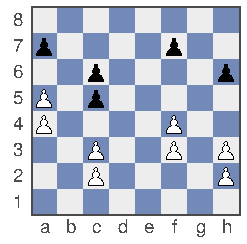
\includegraphics[width=\linewidth]{figures/puzzle71.pdf}
\caption{Puzzle 1: white wins whoever moves first.}
\label{fig:puzzle71}
\end{subfigure}\hfill
\begin{subfigure}{0.32\textwidth}
\centering
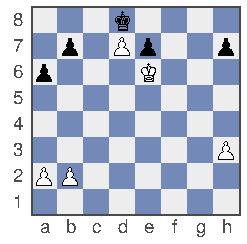
\includegraphics[width=\linewidth]{figures/puzzle72.pdf}
\caption{Puzzle 2: the pawn part is an infinitesimal.}
\label{fig:puzzle72}
\end{subfigure}\hfill
\begin{subfigure}{0.32\textwidth}
\centering
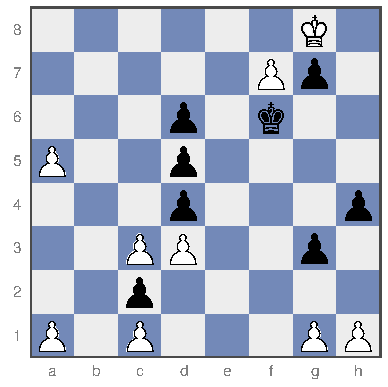
\includegraphics[width=\linewidth]{figures/puzzle73.pdf}
\caption{Puzzle 3 as first drawn: $+\BIG$ (not legal).}
\label{fig:puzzle73}
\end{subfigure}
\caption{Three puzzles (cylinder: files a and h adjacent), Positions 7.1--7.3 of~\cite{Bhattacharjee2025}. Their
exact values are in Table~\ref{tab:puzzles}.}
\label{fig:puzzles}
\end{figure*}

\begin{table}[!t]
\centering
\caption{The Puzzles of Fig.~\ref{fig:puzzles}: Claimed and Exact Values \lab{C2}}
\label{tab:puzzles}
\begin{tabular}{@{}lll@{}}
\toprule
Part & Claimed~\cite{Bhattacharjee2025} & Exact \\
\midrule
1: c-file & $\pm1$ & $\pm1$ \\
1: f-file & $\game{\game{2}{1}}{0}$ & the same (mean $3/4$) \\
1: files h, a & $1$ & $\game{+\BIG}{\star}$ (hot) \\
1: total & $1\pm1+\game{\game{2}{1}}{0}$ & white wins either way \\
2: pawns & $\pm1$ & infinitesimal, mean $0$ \\
2: kings & $0$ & not a zugzwang \\
3: files c, d & $1$ & $\tinyg{1}$ \\
3: total & $2$ & $+\BIG$ before any move \\
\bottomrule
\end{tabular}
\end{table}

\emph{Puzzle 1} (Fig.~\ref{fig:puzzle71}) has three components. On the c-file the first player wins: white
(Left) c3--c4 leaves $1$ and black (Right) c5--c4 leaves $-1$, so $G=\game{1}{-1}=\pm1$. On the f-file white's
f4--f5 leaves $\game{2}{1}$ (white can go on with f5--f6 and keep two spare moves with the f3 pawn, while
black's f7--f6 leaves white one), and black's best, f7--f5, locks the file at $0$. Thus
$G=\game{\game{2}{1}}{0}$, with mean $3/4$, as first found. The earlier analysis goes wrong on files h and a.
White's a5--a6 still wins outright, but black, moving first, plays h6$\times$a5 across the seam and leaves
$\star$, not a loss. So $G=\game{+\BIG}{\star}$: this part is hot, not the number $1$.

The total is still a white win whoever moves first, but for a different reason. By Principle~2 the h/a
component is by far the hottest. White to move plays a5--a6 and wins. Black to move must take on a5 at once,
since any other move allows a5--a6. Then white plays c3--c4 in the next hottest component, and
$1+\star+\game{\game{2}{1}}{0}$ is a white win whoever moves next.

\emph{Puzzle 2} (Fig.~\ref{fig:puzzle72}) has one pawn component, on files h, a and b. The earlier walk-through
finds the right first moves, h3--h4 for white and a6--a5 for black, and the right outcome: whoever moves first
wins. But the value is not $\pm1$; it is an infinitesimal with mean $0$ and temperature $0$. In a sum this
matters: a $\pm1$ would demand an early move, while by Principle~2 this component waits until every hot one is
settled. The king group is that of Fig.~\ref{fig:kinggroup72}, frozen for black only, so with black to move
the model's verdict rests on a final white king move that in chess need not lose. The full ten-man position is
beyond the tablebases, and its real result is open.

\emph{Puzzle 3} (Fig.~\ref{fig:puzzle73}) cannot arise in chess, since four white pawns stand on the first rank.
As drawn it is decided before anyone moves, because the pawns on a5 and f7 are already passed; its king group
is not a tr\'ebuchet either, because f7--f8 promotes. The component on files c and d is still instructive (the
pawns on c1 and c2 block each other). White's best move, c3$\times$d4, leaves $0$. Black's only move is
d4$\times$c3, after which white must answer d3--d4 to lock the files at $0$: if black moved there again,
d5--d4 would leave black the spare move d6--d5, which is $-1$. Thus
\[
G=\ggame{0}{0\mid -1}=\tinyg{1},
\]
a positive infinitesimal, not $1$. A legal copy one rank up, \pos{W c2 c4 d4 / B c3 d5 d6 d7}, has the same
value. In all three puzzles the earlier walk-throughs pick the right winner; what changes is the value, and with
it how each component behaves in a larger sum.

\subsection{When Is the Sum Model Right?}\label{sec:sums-hss}

In chess the first passed pawn ends the game. In a sum it does not: a component with a passed pawn becomes the
integer $\pm\BIG$ and play goes on elsewhere, so a $+\BIG$ can cancel a $-\BIG$. The smallest example is
$\game{\BIG}{0}+\game{0}{-\BIG}$. In chess whoever moves first makes a passed pawn and wins, but the sum is $0$,
a second-player win, for every value of $\BIG$ \lab{P}. We write $S(X)$ for the sum model of a pawn position $X$
and $W(X)$ for the whole-board game, which ends at the first passed pawn anywhere.

\begin{definition}[Hereditary sum safety]\label{def:hss}
A component carries a \emph{threat} for a side if some position reachable from it gives that side a passed
pawn. A position $X$ is \emph{hereditarily sum-safe} (HSS) if no position reachable from $X$ before the first
passed pawn, $X$ included, has two different components that carry threats for opposite sides.
\end{definition}

\begin{theorem}[Sum safety; \lab{P}]\label{thm:hss}
Suppose that $X$ is HSS, that no position with two or more components has a usable en passant right
(condition (E)), and that $\BIG$ exceeds the number of moves either side can make. Then $S(X)$ and $W(X)$ have
the same outcome.
\end{theorem}

\begin{proof}[Proof sketch]
The models can differ only after a passed pawn appears, say for white. By HSS no other component can then give
black a passed pawn, so in the sum white wins by moving in its $+\BIG$ every turn while black runs out of its
fewer than $\BIG$ moves. Induction over the game tree, with (E) to match the moves, gives the theorem.
\end{proof}

In a random sample of $1{,}500$ positions, all $1{,}297$ HSS ones agree. With $\BIG=256$ the move bound always
holds on the 8-rank board, since a side has at most eight pawns and each moves at most six times. The theorem is
about outcomes, not values: a spare move in one component survives a passed pawn in another only in the sum.
Condition (V4) of Theorem~\ref{thm:validity} is the same condition beside a king group. Neither HSS nor (E) can
be dropped.

\begin{figure}[!t]
\centering
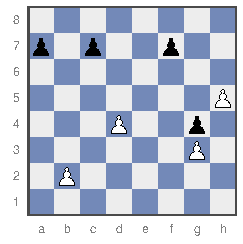
\includegraphics[width=0.5\columnwidth]{figures/sum_counter.pdf}
\caption{Position \pos{W b2 d4 g3 h5 / B a7 c7 f7 g4} (cylinder: files a and h adjacent; en passant off). It is
one component, yet the sum model says that black wins while the whole-board game is a first-player win.}
\label{fig:sum_counter}
\end{figure}

\begin{proposition}[\lab{C2}]\label{prop:sumcounter}
A test of the top-level components alone is not sufficient. On the 8-file cylinder with en passant off,
$X=$\,\pos{W b2 d4 g3 h5 / B a7 c7 f7 g4} (Fig.~\ref{fig:sum_counter}) is a single component, spanning files f
to d across the seam, so such a test passes it. Yet $S(X)$ is a black win whoever starts, while $W(X)$ is a
first-player win.
\end{proposition}

The trouble comes from sums that appear only later in the tree, where components with threats for opposite
sides meet, so the position is not HSS.

\begin{proposition}[\lab{C1}]\label{prop:condE}
Without (E) the sum can be wrong, even in outcome. On the flat $6\times6$ board take \pos{W a4 f4 / B b4 e5},
where white has just played a2--a4, so that black may take b4$\times$a3 en passant on this move only. The whole
board is $\game{0}{-4,\,-3\pm2}$, a first-player win, while the sum of its two components is
$\game{-1\star}{-5\star}$, a black win.
\end{proposition}

In the sum, the en passant right survives moves made in the other component, which chess forbids.

\emph{Two models.} Our CGT engine follows Elkies~\cite{Elkies1996} and adds up components. A separately
written whole-board solver never splits the board and ends the game at the first passed pawn; with splitting
switched off, our engine matches it on every disagreeing case tested. The two models agree on every headline
value of this paper: the $1/8$ and $\upsec\star$ positions in all nine settings, and the seven-pawn $\nim{2}$ under the count rule with the e.p.-aware test. Elsewhere they can differ,
even in outcome: under the opponent race rule with the e.p.-aware test, \pos{W a3 b3 c2 e2 / B a6 c5 d5 e3} is
${\Uparrow}$ as a sum of components but $\nim{2}$ on the whole board. Whenever the two models differ, we say which
one we mean.

\section{Value Atlases: What Only the Cylinder Can Do}\label{sec:atlas}

So far we found each value by hand, one position at a time. With a computer we can instead find the value of
\emph{every} small position and see which values occur at all. We did this twice.
\begin{itemize}
\item \emph{The cylinder atlas} holds every pawn position with at most five pawns on the cylinders
  $\cyl{3},\dots,\cyl{8}$ and the flat boards $\flatb{3},\dots,\flatb{8}$, all with eight ranks:
  $1{,}223{,}689$ positions. They take $10{,}369$ distinct values under the textbook passed-pawn test and
  $10{,}561$ under the e.p.-aware test \lab{C1}; an independent minimax program confirms the textbook outcomes.
\item \emph{The flat census} holds every position with at most six pawns on flat boards of one to four files:
  $231{,}071$ records, standing for $459{,}443$ positions. An independent C solver agrees with ours on every
  record \lab{C2}. We use it for the smallest values (Section~\ref{sec:targets}) and for $\nim{2}$
  (Section~\ref{sec:star2}).
\end{itemize}

\subsection{Which Values Occur}
With at most five pawns, the values without $\pm\BIG$ include the following families.
\begin{itemize}
\item \emph{Nimbers:} only $\star$, and $\nim{2}$ under the textbook test alone (Section~\ref{sec:star2}).
\item \emph{Ups:} ${\uparrow}$, ${\uparrow}\star$, ${\Uparrow}$ and ${\Uparrow}\star$. A single file already holds
  ${\Uparrow}\star$ (Fig.~\ref{fig:basic}(h)).
\item \emph{Fractions:} $\pm1/2$, $\pm1/4$, $\pm3/2$ and $\pm5/2$ on both kinds of board, and $\pm3/4$ only on
  $3$-file cylinders.
\end{itemize}
The six-pawn census adds smaller values, such as $1/8$ and $\upsec\star$ (Section~\ref{sec:targets}).

\begin{figure}[!t]
\centering
\begin{subfigure}[b]{0.36\columnwidth}\centering
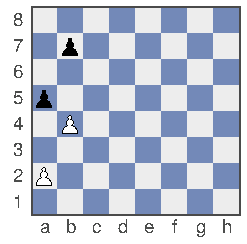
\includegraphics[height=1.25in]{figures/hot3.pdf}
\caption{}
\end{subfigure}\hfill
\begin{subfigure}[b]{0.18\columnwidth}\centering
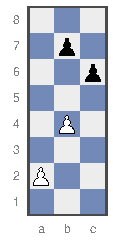
\includegraphics[height=1.25in]{figures/ring3_threequarters.pdf}
\caption{}
\end{subfigure}\hfill
\begin{subfigure}[b]{0.18\columnwidth}\centering
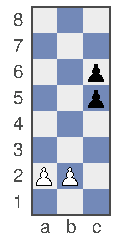
\includegraphics[height=1.25in]{figures/ring3_quarter.pdf}
\caption{}
\end{subfigure}\hfill
\begin{subfigure}[b]{0.22\columnwidth}\centering
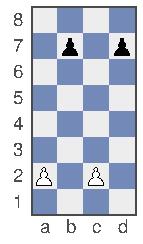
\includegraphics[height=1.25in]{figures/ring4.pdf}
\caption{}
\end{subfigure}
\caption{Hot and cylinder-only pawn values. (a)~White a2, b4 against black a5, b7: $\pm3$, the hottest
position without $\pm\BIG$ (ordinary board; the same on the cylinder). (b)~White a2, b4 against black b7, c6:
$3/4$ (cylinder $\cyl{3}$: files a and c adjacent). (c)~White a2, b2 against black c5, c6: $1/4\pm1/4$
(cylinder $\cyl{3}$). (d)~White a2, c2 against black b7, d7: $\game{3/2\pm1/2}{-3/2\pm1/2}$ under the textbook
test (cylinder $\cyl{4}$: files a and d adjacent).}
\label{fig:hot3}
\end{figure}

\subsection{The Hottest Position}
Apart from $\pm\BIG$, the highest temperature in the atlas (textbook test) is $3$. It is reached by white a2,
b4 against black a5, b7 (Fig.~\ref{fig:hot3}(a)), which is worth $\pm3$ on the ordinary board and on the cylinder
alike \lab{C1}.

Whoever moves first captures. If white (Left) moves first, b4$\times$a5 leaves white's two a-pawns against the lone
black pawn on b7. That pawn is stuck, since either step lets the a5-pawn through, and white is three spare moves
ahead: the value is $3$. If black (Right) moves first, a5$\times$b4 does the same for black and leaves $-3$. Thus
$G=\game{3}{-3}=\pm3$. By Principle~2 (Section~\ref{sec:sums}), this is the first place either player should move.

\subsection{What Only the Cylinder Can Do}
By the cut lemma (Theorem~\ref{thm:cut}), a value that occurs on a cylinder but on no flat board must come from a
\emph{ring}, a position with a pawn on every file. A ring on $n$ files needs at least $n$
pawns, so with five pawns or fewer only $\cyl{3}$, $\cyl{4}$ and $\cyl{5}$ can contribute.

\begin{proposition}[\lab{C1}]\label{prop:cylonly}
Under the textbook test, with at most five pawns, $53$ values free of $\BIG$ occur on some cylinder of width at
most $8$ but on no flat board of width at most $8$. Of these, $40$ come from $3$-file rings and $13$ from $4$-file
rings. Conversely, every value that occurs on a flat board also occurs on some cylinder.
\end{proposition}

Fig.~\ref{fig:hot3}(b)--(d) shows examples. On $\cyl{3}$, white a2, b4 against black b7, c6 is worth $3/4$,
and white a2, b2 against black c5, c6 is worth $1/4\pm1/4$. Both keep their values under the e.p.-aware test.
On $\cyl{4}$, white a2, c2 against black b7, d7 is worth $\game{3/2\pm1/2}{-3/2\pm1/2}$. These are the four
pawns of the $\nim{2}$ candidate of Section~\ref{sec:star2}. On the flat board they make $\nim{2}$ under the
textbook test, and closing the board into a ring turns that into a hot game. Under the e.p.-aware test the
ring is worth $\game{2\pm1}{-2\pm1}$, which is also the e.p.-aware value of the same pawns on the flat board, so
this particular value is no longer cylinder-only.

\subsection{A Correction: Race Rules}
One honest correction. Our first atlas report said that none of the cylinder-only values depends on the race
rule (Section~\ref{sec:rules}). A second, independent computation showed that this is wrong. The $3$-file ring
values do depend on it: $3/4$ becomes $0$ under the mover rule. The $4$-file ring values do not, but they change
when en passant is switched off. So no value is cylinder-only under every combination of race rule and en passant
setting.

\section{Elkies' Small Values}\label{sec:targets}

Elkies~\cite{Elkies1996} found fractions, ups and tinies in chess endgames on the ordinary board. The flat census
lets us ask which smaller values of this kind occur with at most six pawns, and where. Each halving is one more
step: $1/8=\game{0}{1/4}$, $1/16=\game{0}{1/8}$ and $1/32=\game{0}{1/16}$. Up-second and the tinies were
defined in Section~\ref{sec:rules}; adding $\star$ to up-second gives $\upsec\star=\game{0,\star}{{\downarrow}}$.

\begin{table}[!t]
\caption{Elkies' Targets in the Flat Census}
\label{tab:targets}
\centering
\begin{tabular}{@{}llcc@{}}
\toprule
Target & Form & Textbook & E.p.-aware \\
\midrule
$1/8$ & $\game{0}{1/4}$ & $13$ & $9$ \\
$1/16$ & $\game{0}{1/8}$ & $3$ & $2$ \\
$1/32$ & $\game{0}{1/16}$ & $1$ & $0$ \\
$\upsec$ & $\game{0}{{\downarrow}\star}$ & $5$ & $2$ \\
$\upsec\star$ & $\game{0,\star}{{\downarrow}}$ & $10$ & $10$ \\
$\tinyg{1}$ & $\ggame{0}{0\mid -1}$ & $13$ & $16$ \\
$\tinyg{x}$, $x\notin\mathbb{Z}$ & $\ggame{0}{0\mid -x}$ & $0$ & $0$ \\
\bottomrule
\end{tabular}

\smallskip
\parbox{\columnwidth}{\footnotesize Number of positions of each exact value; flat boards of one to four files,
at most six pawns, count rule, en passant on. Every counted identity was confirmed by an independent solver
\lab{C2}.}
\end{table}

Table~\ref{tab:targets} counts the positions of each target under both passed-pawn tests. For every counted
position $G$ and target $T$, an independent C solver checked that $G-T=0$. The e.p.-aware test thins out the
smallest numbers: $1/32$ disappears and $1/16$ drops to two positions. Up-second falls from five positions to two, while $\upsec\star$ is untouched and $\tinyg{1}$ rises from $13$ to $16$.

\begin{figure*}[!t]
\centering
\begin{subfigure}[b]{0.3\textwidth}\centering
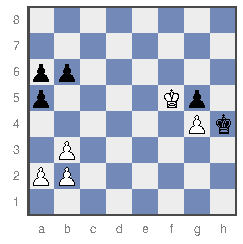
\includegraphics[width=1.62in]{figures/eighth.pdf}
\caption{}
\end{subfigure}\hfil
\begin{subfigure}[b]{0.3\textwidth}\centering
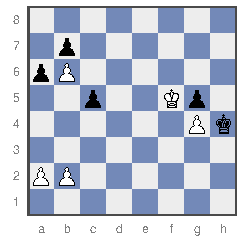
\includegraphics[width=1.62in]{figures/upsecstar.pdf}
\caption{}
\end{subfigure}\hfil
\begin{subfigure}[b]{0.3\textwidth}\centering
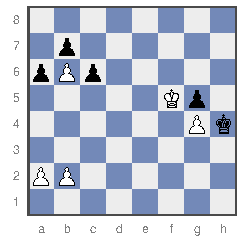
\includegraphics[width=1.62in]{figures/tiny1.pdf}
\caption{}
\end{subfigure}
\caption{Elkies' small values beside the tr\'ebuchet (white Kf5 and g4, black Kh4 and g5), each a legal
10-man position (ordinary board). (a)~$1/8$: white a2, b2, b3 against black a5, a6, b6. (b)~$\upsec\star$:
white a2, b2, b6 against black a6, b7, c5. (c)~$\tinyg{1}$: white a2, b2, b6 against black a6, b7, c6.}
\label{fig:eighth}
\end{figure*}

\subsection{An Eighth That Can Happen in a Game}

\begin{theorem}[\lab{C2}]\label{thm:eighth}
In the pawn model, white a2, b2, b3 against black a5, a6, b6 has value exactly $1/8$. This holds in all nine
settings (the three race rules, each with en passant off, with the textbook test and with the e.p.-aware test)
and for every assignment of outcomes to its race positions.
\end{theorem}

So this $1/8$ does not depend on how races are settled at all. A third, separately written solver agrees in all
nine settings.

Let's see why (Fig.~\ref{fig:eighth}(a)). If white (Left) moves first, a2--a4 locks the a-file and leaves the
zero game. The quieter a2--a3 only reaches $\star$, a reversible move, since black answers it back to $0$. The
move b3--b4 is bad: black answers to $-3$. If black (Right) moves first, b6--b5 leaves $1/4$, and a5--a4 is bad.
Thus $G=\game{0}{1/4}=1/8$.

This pawn structure can arise in a real game. From the starting position, c2$\times$b3, a7--a5, b7$\times$a6 and c7$\times$b6
produce it. Its mirror image, white a2, a3, b2 against black a6, b5, b6, has the same value but cannot arise:
the pawn on a3 could only have come from b2, which is still occupied. Beside the tr\'ebuchet, the $1/8$ becomes
the legal 10-man position of Fig.~\ref{fig:eighth}(a). Whether it keeps its value with real kings is the subject
of Section~\ref{sec:real}.

\subsection{Up-Second Star and Tiny 1}
White a2, b2, b6 against black a6, b7, c5 (Fig.~\ref{fig:eighth}(b)) is $\upsec\star$ in all nine settings
\lab{C2}. If white moves first, a2--a4 leaves $0$ and a2--a3 leaves $\star$. If black moves first, a6--a5 leaves
${\downarrow}$. Thus $G=\game{0,\star}{{\downarrow}}=\upsec\star$.

Now move the black c-pawn back to c6 (Fig.~\ref{fig:eighth}(c)). If white moves first, a2--a3 leaves $0$. If
black moves first, a6--a5 leaves $-1/2\pm1/2=\game{0}{-1}$. Black's other move, c6--c5, reaches exactly the
$\upsec\star$ position above, and it is dominated, since $\game{0}{-1}\le\upsec\star$. Thus
$G=\ggame{0}{0\mid -1}=\tinyg{1}$ with en passant on, under every race rule \lab{C2}. Unlike the Tiny~1 of
Section~\ref{sec:basic}, which lives on the a- and h-files across the seam, this one fits on the ordinary board
beside the tr\'ebuchet.

\subsection{Two Textbook Results That Do Not Survive}
Under the textbook test we had found a $1/8$ at white a2, b2, d2 against black a5, c4, d7, which we singled out
as reachable, and an exact $\upsec$ at white a3, c5, d4 against black a7, b7, d7. Under the e.p.-aware test the
first is worth $-3/2\pm3/2$ and the second $\game{3/4}{{\downarrow}\star}$. The two tests differ only just after a
double step that the opponent may still take en passant, so both values rested on such a pawn being counted as
passed. This is why we ask for values that, like Theorem~\ref{thm:eighth}, hold in all nine settings.

\section{The \texorpdfstring{$\nim{2}$}{*2} Question}\label{sec:star2}

The nimber $\nim{2}$ is a nim heap of size two: whoever moves may go to $0$ or to $\star$. The $\nim{2}$
question of Section~\ref{sec:intro} asks whether a position with only kings and pawns on a board with eight
ranks can have this value. In this section we show that the one $\nim{2}$ among small positions is an artifact
of en passant, that no $\nim{2}$ exists with six pawns or fewer, and that $\nim{2}$ comes back with seven.

\subsection{The Textbook Candidate}

\begin{figure}[!t]
\centering
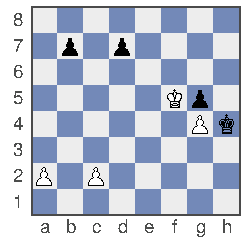
\includegraphics[width=0.7\columnwidth]{figures/star2_textbook.pdf}
\caption{Textbook $\nim{2}$ candidate \pos{W a2 c2 / B b7 d7}, with the kings frozen by the tr\'ebuchet on
files f--h (ordinary board). It is $\nim{2}$ under the textbook passed-pawn test and $\game{2\pm1}{-2\pm1}$
under the e.p.-aware test.}
\label{fig:star2_textbook}
\end{figure}

Fig.~\ref{fig:star2_textbook} shows \pos{W a2 c2 / B b7 d7} on files a--d, with the kings frozen by the
tr\'ebuchet on files f--h. Under the textbook passed-pawn test and the count rule, it is the only position of
value $\nim{k}$ with $k\ge2$ in the flat census. If white (Left) moves first, a2--a4 leaves $\star$ and c2--c4
leaves the zero game; the single steps a2--a3 and c2--c3 are worse. The position is symmetric (turn the board
around and swap the colors), so black (Right) has the same choice: d7--d5 leaves $\star$ and b7--b5 leaves $0$.
Thus $G=\game{0,\star}{0,\star}=\nim{2}$. The value is the same under the mover rule and with e.p.\ off, and it is
$0$ under the opponent rule \lab{C2}.

The weak point is black's plan b7--b5 and b5--b4. The textbook test answers b5--b4 with a2--a4: no black pawn
stands in front of the a-pawn, so the test calls it passed and scores $+\BIG$. In chess, black simply plays b4$\times$a3
en passant. Under the e.p.-aware test of Section~\ref{sec:rules}, the position after b5--b4,
\pos{W a2 c2 / B b4 d7}, is no longer a white win but a black one. So b7--b5 is worth $-2\pm1$ for black and, by
symmetry, c2--c4 is worth $2\pm1$ for white. The other moves, such as a2--a4 and d7--d5 (both still to $\star$),
are dominated or reversible. Hence
\begin{equation}
G=\game{2\pm1}{-2\pm1}\qquad\lab{C2},
\end{equation}
a hot game with mean $0$ and temperature $2$. The candidate's $\nim{2}$ rested on one double step, a2--a4 past
a black pawn on b4, that the textbook test counts as passed one move too early.

\subsection{No \texorpdfstring{$\nim{2}$}{*2} With Six Pawns or Fewer}

\begin{theorem}[Census; \lab{C2}]\label{thm:census}
Consider the flat census: ordinary boards with $8$ ranks and $1$ to $4$ files, with at most six pawns
($231{,}071$ records standing for $459{,}443$ positions). Under the count rule with the e.p.-aware test and
e.p.\ on, no position has value $\nim{k}$ with $k\ge2$. The census has $6{,}724$ positions of value $0$ and
$4{,}042$ of value $\star$.
\end{theorem}

Three independent programs give this result (Section~\ref{sec:verify}). Our CGT engine and a separate C
solver, which tests whether $G+\nim{k}$ is a second-player win, agree on every record. A third solver, written
from the rules alone, finds no $\nim{k}$ with $2\le k\le 292$ among $793{,}299$ labeled placements. Every
position in scope has birthday at most $292$ (at most $36$ pawn moves before a decided position of birthday
$\BIG=256$), so no larger nimber can occur. Under the textbook test the same census has $6{,}470$ zeros,
$3{,}891$ stars and the one $\nim{2}$ above. The e.p.-aware test removes that $\nim{2}$ and creates none, so in
this scope the only route to $\nim{2}$ was the en passant artifact.

\subsection{\texorpdfstring{$\nim{2}$}{*2} Returns With Seven Pawns}

\begin{theorem}[$\nim{2}$ with seven pawns; \lab{C2}]\label{thm:star2seven}
Under the count rule with the e.p.-aware test and e.p.\ on, position~A, \pos{W a4 b3 d2 d3 / B a7 b7 c5}, and
position~B, \pos{W b4 c2 d2 / B a6 a7 c6 d5}, both on files a--d of the ordinary board, have value $\nim{2}$.
Both are also $\nim{2}$ under the mover rule and under the textbook test. Neither is $\nim{2}$ with e.p.\ off or
under the opponent rule. Both embed legally beside the tr\'ebuchet on files f--h.
\end{theorem}

Three programs give $\nim{2}$ in every setting the theorem claims: our CGT engine (on 4- and 8-file boards), the
C scanner that found the two positions, and the independent whole-board solver.

\begin{figure}[!t]
\centering
\begin{subfigure}{0.48\columnwidth}\centering
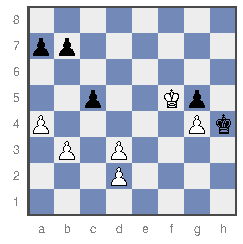
\includegraphics[width=\linewidth]{figures/star2_seven_a.pdf}
\caption{Position A}\label{fig:star2_seven_a}
\end{subfigure}\hfill
\begin{subfigure}{0.48\columnwidth}\centering
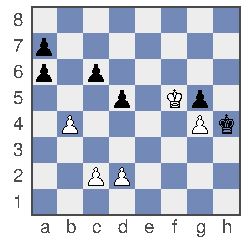
\includegraphics[width=\linewidth]{figures/star2_seven_b.pdf}
\caption{Position B}\label{fig:star2_seven_b}
\end{subfigure}
\caption{Seven-pawn positions of value $\nim{2}$ (count rule, e.p.-aware test), each beside the tr\'ebuchet on
files f--h (ordinary board). (a) Position A, \pos{W a4 b3 d2 d3 / B a7 b7 c5}. (b) Position B,
\pos{W b4 c2 d2 / B a6 a7 c6 d5}.}
\label{fig:star2_seven}
\end{figure}

In position A (Fig.~\ref{fig:star2_seven_a}), if white (Left) moves first, a4--a5 leaves the zero game. The move
d3--d4 attacks c5, and every black reply except c5$\times$d4 loses at once; after c5$\times$d4, white continues b3--b4 and
reaches $\star$. So d3--d4 is a reversible move, and it counts as a move to $\star$. White's last move, b3--b4,
loses to c5$\times$b4, which gives black a passed pawn. If black (Right) moves first, a7--a5 leaves $0$ and b7--b6
leaves $\star$. Black's other moves are worse: a7--a6 and b7--b5 are dominated, and c5--c4 loses the pawn to a
capture on c4 that frees white's d-pawn. Thus $G=\game{0,\star}{0,\star}=\nim{2}$.

In position B (Fig.~\ref{fig:star2_seven_b}), if white moves first, d2--d4 leaves $0$ and c2--c3 leaves
$\star$. The moves d2--d3 and c2--c4 are dominated, and b4--b5 loses to a6$\times$b5. Black has three moves. d5--d4
leaves $0$. The move a6--a5 attacks b4: every white reply except b4$\times$a5 loses at once, and after b4$\times$a5 black
continues c6--c5 and reaches $\star$. So, as in A, a reversible move counts as a move to $\star$. Finally,
c6--c5 loses to b4$\times$c5. Thus $G=\nim{2}$ again.

\begin{table}[!t]
\centering
\caption{Values of the Three $\nim{2}$ Positions in the Model Settings}
\label{tab:star2_settings}
\footnotesize
\setlength{\tabcolsep}{4pt}
\begin{tabular}{@{}lccc@{}}
\toprule
Race rule, passed-pawn test & Candidate & A & B\\
\midrule
count, e.p.-aware & $\game{2\pm1}{-2\pm1}$ & $\nim{2}$ & $\nim{2}$\\
mover, e.p.-aware & $\game{2\pm1}{-2\pm1}$ & $\nim{2}$ & $\nim{2}$\\
count or mover, textbook & $\nim{2}$ & $\nim{2}$ & $\nim{2}$\\
count or mover, e.p.\ off & $\nim{2}$ & not $\nim{2}$ & not $\nim{2}$\\
opponent, textbook or e.p.\ off & $0$ & not $\nim{2}$ & not $\nim{2}$\\
\bottomrule
\end{tabular}
\end{table}

Table~\ref{tab:star2_settings} compares the settings (e.p.\ on unless stated; every entry \lab{C2}). The
candidate and the new positions fail in opposite places. The candidate needs the textbook test but survives
e.p.\ off. Positions A and B do not depend on the passed-pawn test at all, but they need en passant: with e.p.\
off neither is $\nim{2}$.

\begin{figure}[!t]
\centering
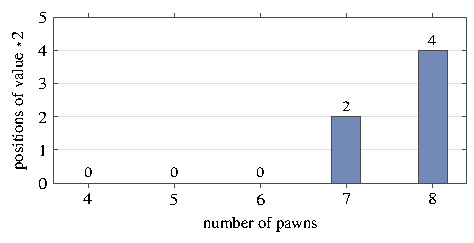
\includegraphics[width=\columnwidth]{figures/star2_by_pawns.pdf}
\caption{Number of $\nim{2}$ positions by number of pawns, on ordinary boards of width at most four (count rule,
e.p.-aware test). The bars for four to six pawns are \lab{C2}. The bars for seven and eight pawns are \lab{C1}
as counts, and every position they count was re-checked \lab{C2}.}
\label{fig:star2_by_pawns}
\end{figure}

\subsubsection{Scope}
Fig.~\ref{fig:star2_by_pawns} counts $\nim{2}$ positions by number of pawns on ordinary boards of width at most
four. With four to six pawns there are none (Theorem~\ref{thm:census}). With seven pawns there are exactly the
two above, and with eight pawns there are four. These two counts come from one exhaustive scan of
$5{,}503{,}282$ root positions, so as claims of completeness they are \lab{C1}; every position the scan reported
was re-checked by our engine \lab{C2}. Theorems~\ref{thm:census} and~\ref{thm:star2seven} together show that
seven is the least number of pawns in a $\nim{2}$ on ordinary boards of width at most four \lab{C2}.

\subsubsection{Five files}
We also know three eight-pawn positions on five files that are $\nim{2}$ on the ordinary board \lab{C2}, both
as a sum of components and on the whole board (Section~\ref{sec:sums}): \pos{W a3 b3 c2 e2 / B a6 c5 d5 e3},
\pos{W a4 b3 c2 d2 / B a7 b6 c7 e4} and \pos{W a6 b4 c4 e3 / B a7 c7 d6 e6}. They come from a scan of
eight-pawn rings on the 5-file cylinder $\cyl{5}$, which finds $14$ rings of value $\nim{2}$ \lab{C1}, each
confirmed by our engine. Opened onto files a--e of the ordinary board, $11$ of the $14$ change value and only
these three stay $\nim{2}$. No $\nim{3}$ or higher nimber occurs under the count rule with the e.p.-aware test
in any scope we searched \lab{C1}.

\subsubsection{What this answers}
Within the model, with the kings frozen by the tr\'ebuchet, the count rule and the e.p.-aware test, the
$\nim{2}$ question has a positive answer: there are king-and-pawn positions on the ordinary $8\times8$ board of
value $\nim{2}$. Elkies' higher nimbers live on larger boards~\cite{Elkies2002}. Positions A and B use four files of
the 8-rank board, no officers and seven pawns, and they hold under the stricter passed-pawn test that removed the
candidate. The answer has limits: it fails under the opponent rule and with e.p.\ off, the completeness counts
for seven and eight pawns are \lab{C1}, and the value is a model value. Whether real chess agrees is the
subject of Section~\ref{sec:real}.

\section{From the Model to Real Chess}\label{sec:real}

A model value rests on conventions: a passed pawn wins, the kings stay frozen, and a race between two passed
pawns is settled by a fixed rule. None of these is exact chess. To test a value against chess, we keep the
model's tree of pawn moves and replace only its leaves by real results.

\begin{definition}[Real-chess oracle value]\label{def:oracle}
Let $X$ be a pawn component on the ordinary board beside the tr\'ebuchet. An \emph{end position} of the model tree of
$X$ is the first position on a line of play in which some side has a passed pawn. Each end position has two sides,
white to move and black to move. Replace each end position by $+\BIG$ if white wins it in real chess with either
side to move, by $-\BIG$ if black does, and otherwise (the side to move wins, the second player wins, or a side
is drawn) by a game $t$ with $-2\BIG\le t\le 2\BIG$ fixed in advance, called a \emph{treatment}. The canonical
value of the resulting tree is the \emph{oracle value} $O(X)$.
\end{definition}

The real results come from the Lichess Syzygy tablebase~\cite{LichessTB} for at most seven men, and from
tablebase-backed search and our king-and-pawn solver (Section~\ref{sec:kings}) beyond that. End positions with more
than seven men are slow to resolve, so we need a way to bound $O(X)$ while some of them are unknown.

\begin{lemma}[Sandwich; \lab{P}]\label{lem:sandwich}
Let $O^-$ and $O^+$ be the values obtained when every end position that is not known to be $+\BIG$ or $-\BIG$ is
replaced by $-2\BIG$ and by $+2\BIG$, respectively. Then $O^-\le O(X)\le O^+$ for every treatment and every real
outcome of the unknown end positions. If $O^-=O^+$, then $O(X)$ is certified.
\end{lemma}
\begin{proof}
Raising an option never lowers a game: if $H\le H'$, then a game with $H$ among its options is at most the same
game with $H'$ in its place~\cite{Siegel2013}. Every leaf of the tree lies between $-2\BIG$ and $2\BIG$, so by
induction from the leaves to the root, $O^-\le O(X)\le O^+$.
\end{proof}

We also use the \emph{stops} of a game: the numbers reached when white or black moves first and both sides play
until a number appears. Both stops of $0$ and of $\nim{2}$ are $0$.

\subsection{The Textbook Candidate in Real Chess}

\begin{theorem}[Candidate in real chess; end positions \lab{C2}, values \lab{C1}]\label{thm:oracle-cand}
For the candidate \pos{W a2 c2 / B b7 d7} beside the tr\'ebuchet (Fig.~\ref{fig:star2_textbook}):
\begin{enumerate}
\item[(a)] In real chess the side to move wins, with either side to move. With black to move, only 1\ldots b5 wins.
  With white to move, 1.c4 wins and every king move loses.
\item[(b)] In the e.p.-aware tree, $O\ne\nim{2}$ and $O\ne0$ under every treatment: the bounds force white's stop
  to be at least $1$ and black's stop to be at most $-1$.
\item[(c)] If draws count as wins for black, then $O=\game{2\pm1}{-2\pm1}$ exactly, in both the textbook and the
  e.p.-aware tree.
\end{enumerate}
\end{theorem}

Part (a) is proved by explicit certificates checked against the tablebase. So real chess agrees with
$\nim{2}$ on the outcome, a first-player win, and the winning first moves found, 1.c4 and 1\ldots b5, are the
ones the model predicts. It disagrees on the value. In the e.p.-aware tree the two stops differ under every
treatment, so the oracle value is a hot game, as the e.p.-aware model value $\game{2\pm1}{-2\pm1}$ of
Section~\ref{sec:star2} is. In the textbook tree, $\nim{2}$ is excluded only when draws count as wins for one
side. The textbook $\nim{2}$ therefore does not survive real chess.

A few other positions are $\nim{2}$ under a single non-default setting, and each needs $10$ men beside the
tr\'ebuchet. One of them, \pos{W a3 b3 c2 / B b5 b7 c6}, is refuted: its oracle value is positive under every
treatment \lab{C2}. For three others, the tablebase contradicts the race verdicts that their $\nim{2}$ needs,
but their oracle values cannot be pinned with seven-man tablebases.

\subsection{Towards a Real-Chess \texorpdfstring{$1/8$}{1/8}}

The $1/8$ position of Section~\ref{sec:targets}, \pos{W a2 b2 b3 / B a5 a6 b6} beside the tr\'ebuchet
(Fig.~\ref{fig:eighth}(a)), has $10$ men. We computed its oracle value as far as the end positions allow.
\begin{itemize}
\item All $306$ end-position sides with at most seven men are resolved by the tablebase: $283$ agree with the
  model, $5$ disagree and $2$ are draws.
\item A greedy search for a smallest decisive set then left eight open end positions that matter, five with
  eight men and three with nine. Resolving eight-man sides gave seven agreements and one disagreement: with
  black to move in \pos{W a3 a5 / B b4 b5}, black wins, although the model scores a white win.
\item After these results the bounds were $-1/2\le O\le 3/8\pm1/8$, and four decisive end positions
  remained: three with nine men, and \pos{W b2 b5 / B a5 b4} with eight. Our king-and-pawn solver showed that
  white wins the last with white to move, as the model says. Each of the other seven sides was then needed on
  its own: if any one went against the model, the lower bound would fall to $0$, ${\uparrow}{\star}$ or below.
\item The solver then settled all six sides of the three nine-man positions exactly, and all six agree with
  the model.
\end{itemize}

\begin{proposition}[Status of $1/8$; \lab{C1}]\label{prop:eighth-real}
For the $1/8$ position beside the tr\'ebuchet, the exact results give $0\le O\le 1/8$. If black, to move in
\pos{W b2 b5 / B a5 b4}, loses, as the model assigns, then $O=1/8$ exactly, whatever the other open end
positions do.
\end{proposition}

The tablebase and tablebase-backed results are \lab{C2}; the king-and-pawn solver results and the values
are \lab{C1}. The solver runs allow queen promotions only, so a full certificate
also needs the under-promotions. The value $1/8$ has survived every real-chess test so far, including one
disagreement at a decisive end position. If the last side goes as the model says, this gives a king-and-pawn
position on the $8\times8$ board whose oracle value is $1/8$, conditional only on the king freeze.

\subsection{The Seven-Pawn \texorpdfstring{$\nim{2}$}{*2} in Real Chess}

Positions A and B have $11$ men beside the tr\'ebuchet, and the five-file witnesses have $12$. Their oracle
values are open. Computing them needs end positions beyond the reach of the seven-man tablebase, so it is
a task for the king-and-pawn solver (Section~\ref{sec:conclusion}). Until then, the $\nim{2}$ of
Theorem~\ref{thm:star2seven} is a model value.

\section{Mating Without Corners: Tablebases}\label{sec:tb}

Up to now our boards have held only kings and pawns. Here we bring in the pieces and ask a classical
question: without corners, which material can still force mate? We computed every
4-man pawnless tablebase on the plane (the ordinary board), on the cylinder (files a and h adjacent) and on the torus (ranks 1
and 8 adjacent as well). Chess on these boards is an old variant~\cite{Pritchard}, but we found no earlier
tablebase for them.

\emph{Rules.} Every piece moves as usual and wraps round each glued edge. A rook, bishop or queen stops when
its ray comes back to its own square, so a rook on an empty rank cannot travel round it and ``pass''. There
is no castling and no fifty-move rule. Stalemate and bare kings are draws, and when black captures, play
continues in the smaller table. A position is legal when the kings are not adjacent, across the seams
included, and the side not to move is not in check. Both sides of the board have even length, so the
coloring of the squares survives the gluing, and ``bishops on opposite colors'' still makes sense.

\emph{Verification.} Two retrograde solvers, written independently from these rules, agree on every position
of all 24 tables, about 607 million values with either side to move \lab{C2}. One of them also re-derives
every value from its children and checks the board's symmetries on every position. On the plane both
reproduce the known longest mates: KQK 10, KRK 16, KBBK 19 and KBNK 33 moves.

\begin{table}[!t]
\centering
\caption{Four-Man Pawnless Endings: Share Won With White to Move and Longest Forced Mate in Moves
\lab{C2}. KBBK Has Bishops on Opposite Colors}
\label{tab:tb}
\footnotesize
\setlength{\tabcolsep}{4.5pt}
\begin{tabular}{@{}lrrrrrr@{}}
\toprule
& \multicolumn{2}{c}{Plane} & \multicolumn{2}{c}{Cylinder} & \multicolumn{2}{c}{Torus} \\
\cmidrule(lr){2-3}\cmidrule(lr){4-5}\cmidrule(l){6-7}
Material & Won (\%) & Mate & Won (\%) & Mate & Won (\%) & Mate \\
\midrule
KQK  & 100    & 10 & 100    & 10 & 0      & --- \\
KRK  & 100    & 16 & 2.80   & 3  & 0      & --- \\
KBBK & 99.98  & 19 & 100    & 14 & 0      & --- \\
KBNK & 99.51  & 33 & 0.0245 & 2  & 0      & --- \\
KNNK & 0.0107 & 1  & 0.0077 & 1  & 0      & --- \\
KRBK & 100    & 16 & 99.74  & 13 & 0.0218 & 1   \\
KRRK & 100    & 7  & 100    & 8  & 100    & 7   \\
KQRK & 100    & 6  & 100    & 5  & 100    & 5   \\
\bottomrule
\end{tabular}
\end{table}

\begin{figure}[!t]
\centering
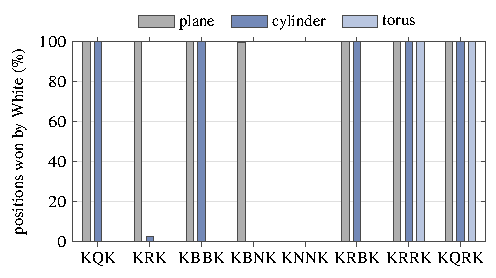
\includegraphics[width=\columnwidth]{figures/tb_bars.pdf}
\caption{Share of legal positions won by white with white to move, for each 4-man pawnless ending on the
plane, the cylinder and the torus (Table~\ref{tab:tb}). On the torus only KRRK and KQRK win; the KRBK
bar (0.0218\%) is too small to see.}
\label{fig:tb_bars}
\end{figure}

Table~\ref{tab:tb} and Fig.~\ref{fig:tb_bars} give the results. The queen does not notice the seam: KQK
is won from every position on the cylinder, in at most 10 moves, as on the plane. The rook and the minor pieces
do notice it.

\emph{KRK and KBNK are draws on the cylinder.} The first and eighth ranks are still edges, but each is now a
closed loop with no corner in it. The rook wins only 2.80\% of the positions, all of them mates in at most
three moves. The longest is Ka3, Rb2 against Ka1: 1.~Rb3 Kh1 2.~Rg3 Ka1
3.~Rg1\#. On the cylinder h1 and h2 are neighbors of a1, so the rook covers h1 along the first rank and the
white king covers h2 across the seam. The bishop and knight win only 0.0245\% of the positions, within two
moves; on the plane their mate needs a corner of the bishop's color, and the cylinder has none.

\emph{Bishops on opposite colors win every position on the cylinder}, in at most 14 moves against 19 on
the plane. Here the seam helps the attacker: a diagonal winds round the cylinder, so from every square of the
first rank a bishop reaches the eighth. The longest line ends in Ke6, Be1, Bf1 against Ke8. The bishop on f1
gives check along f1--h3--a4--e8, once round the board, and the bishop on e1 covers d8 and f8 along its two diagonals.

\emph{On the torus no single piece, and no pair weaker than two rooks, can force mate.} KQK, KRK, KBBK, KBNK and KNNK
are not won from a single position. KRBK wins 0.0218\% of the positions, and every one of these wins is a
mate in one. The bishop pair even has mating positions on the torus, but none of them can arise from a
legal white move. Only KRRK and KQRK win, from every position.

\subsection{King and Pawn Against King}\label{sec:kpk}

We solved every legal KPK position on the $8\times8$ plane and cylinder twice: with the king-and-pawn solver
used for the tr\'ebuchet (all four promotions) and with a separately written KPK solver (queen promotion
only). On the cylinder the two agree on all 326,640 positions. On the plane they differ on exactly 6, the
positions in which only promotion to a rook avoids stalemate, such as Ka4, Pb7 against Ka6 \lab{C2}.
Table~\ref{tab:kpk} gives the counts and Fig.~\ref{fig:kpk_bars} the shares won. The cylinder has fewer
legal positions because the kings may not stand next to each other across the seam.

\begin{table}[!t]
\centering
\caption{King and Pawn Against King: Legal Positions and white Wins on the $8\times8$ Plane and Cylinder
\lab{C2}}
\label{tab:kpk}
\footnotesize
\begin{tabular}{@{}lrrrr@{}}
\toprule
& \multicolumn{2}{c}{White to move} & \multicolumn{2}{c}{Black to move} \\
\cmidrule(lr){2-3}\cmidrule(l){4-5}
Board & Legal & White wins & Legal & White wins \\
\midrule
Plane    & 163,328 & 124,960 & 168,024 & 97,604 \\
Cylinder & 160,656 & 126,736 & 165,984 & 92,760 \\
\bottomrule
\end{tabular}
\end{table}

\begin{figure}[!t]
\centering
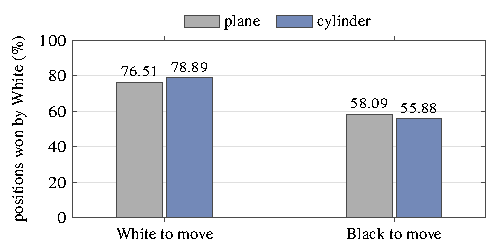
\includegraphics[width=\columnwidth]{figures/kpk_bars.pdf}
\caption{Share of legal KPK positions won by white, plane against cylinder, with white and with black to
move (Table~\ref{tab:kpk}). The seam raises white's share with white to move and lowers it with black to
move.}
\label{fig:kpk_bars}
\end{figure}

\begin{figure}[!t]
\centering
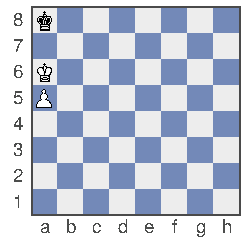
\includegraphics[width=0.5\columnwidth]{figures/kpk_rookpawn.pdf}
\caption{Ka6, Pa5 against Ka8 (cylinder: files a and h adjacent). White wins with either side to move. On
the ordinary board it is the rook-pawn draw with either side to move.}
\label{fig:kpk_rookpawn}
\end{figure}

On a cylinder every file is a center file, so there are no rook pawns.
Fig.~\ref{fig:kpk_rookpawn} shows the classic rook-pawn draw: on the plane the black king cannot be driven
out of the corner without stalemate. On the cylinder we may shift every man four files to the right, and
the position becomes Ke6, Pe5 against Ke8, the textbook win, whoever is to move, with the king on the sixth rank in
front of its pawn. Back on the a-file, with black to move, play goes 1\ldots~Kb8 2.~Kh7! Kb7 3.~a6+, and the pawn
promotes under the king, which guards a7 and a8 from h7 across the seam.

Of the 326,640 positions legal on both boards, 16,538 flat draws become cylinder wins, among them
that of Fig.~\ref{fig:kpk_rookpawn}. The seam also
helps the defender, since a king on the h-file now stands beside an a-pawn: 15,930 flat wins become
cylinder draws. Zugzwang, the engine of the tr\'ebuchet, is more common on the cylinder. The cylinder has 216
mutual zugzwangs, positions in which white to move only draws but black to move loses, against 160 on the
plane \lab{C2}.

\section{Dawson's Chess on the Cylinder}\label{sec:dawson}

On a cylinder every file is alike, so after the first move a ring of files should open into an ordinary
strip. The earlier study~\cite{Bhattacharjee2025} used this idea on Dawson's chess and found that a ring of
$n$ files reduces to a strip of $n-3$. The idea is right, but the game was stated incorrectly there, so we
restate the rules and redo the analysis.

\begin{figure}[!t]
\centering
\begin{subfigure}{0.48\columnwidth}
\centering
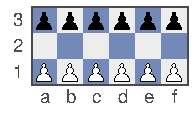
\includegraphics[width=\linewidth]{figures/dawson_strip.pdf}
\caption{}
\label{fig:dawson_strip}
\end{subfigure}\hfill
\begin{subfigure}{0.48\columnwidth}
\centering
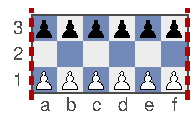
\includegraphics[width=\linewidth]{figures/dawson_ring.pdf}
\caption{}
\label{fig:dawson_ring}
\end{subfigure}
\caption{Starting position of Dawson's chess on six files. (a) Flat $3\times6$ strip (ordinary board).
(b) $3\times6$ cylinder; the arrow marks the seam, so files f and a are adjacent.}
\label{fig:dawson_boards}
\end{figure}

\begin{figure*}[!t]
\centering
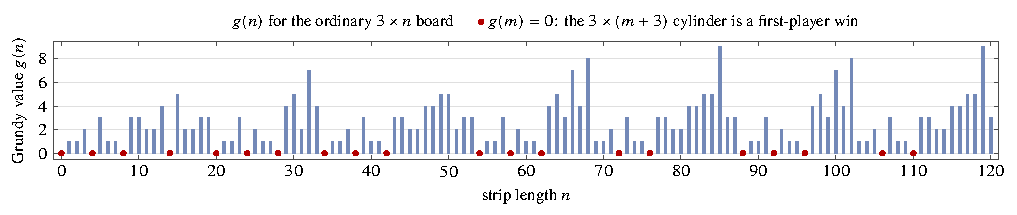
\includegraphics[width=\textwidth]{figures/dawson_grundy.pdf}
\caption{Grundy values $g(n)$ of Dawson's chess on the flat $3\times n$ board (octal game
$\mathbf{0.137}$) for $n\le120$. The dots (red) mark $g(m)=0$, where the flat $3\times m$ board is a
second-player win and the $3\times(m+3)$ cylinder is a first-player win (Theorem~\ref{thm:ring}).}
\label{fig:dawson_grundy}
\end{figure*}

\emph{Rules.} Dawson's chess~\cite{Dawson1935} is played on a $3\times n$ board
(Fig.~\ref{fig:dawson_boards}). White pawns fill rank~1, black pawns fill rank~3, and rank~2 is empty.
Pawns move and capture as in chess, and captures are compulsory. There is no room for a double step, so
there is no en passant, and no pawn ever promotes. Under normal play the last player to move wins. Dawson
himself posed the misère form, which we return to below.

Let us see what one move does. Call a file \emph{untouched} if it still has its white pawn on rank~1, its
black pawn on rank~3 and an empty square between them. Suppose white plays c1--c2 when the b- and d-files are
untouched. The pawn on c2 attacks b3 and d3, so black must capture, say b3$\times$c2. That pawn attacks b1 and d1,
so white must recapture, say d1$\times$c2. Black recaptures with d3$\times$c2 and white with b1$\times$c2. After the push and four
forced captures, the b- and d-files are empty, the c-file holds a blocked pair, and black is to move. Empty
and blocked files never change again, because a pawn can enter a file only by capturing on it. At the end of
a row the same push takes three plies and empties its one neighbor, and a push on a file with no untouched
neighbor is simply blocked.

So a strip of $n$ untouched files is a row of $n$ pins in which a move removes one pin together with its
surviving neighbors. This is the octal game $\mathbf{0.137}$ of Guy and Smith~\cite{GuySmith1956,WinningWays}.
Both players have the same moves, so the game is impartial and each strip has a Grundy value $g(n)$:
$g(0)=0$, $g(1)=1$ and, for $n\ge2$,
\begin{equation}\label{eq:dawson}
g(n)=\operatorname{mex}\bigl(\{g(n-2)\}\cup\{g(a)\oplus g(b) : a+b=n-3\}\bigr),
\end{equation}
where $g(n-2)$ comes from a push on an end file, $\oplus$ is the bitwise exclusive or, and mex is the least
non-negative integer not in the set. A board with several strips has the nim-sum of their values, and the
first player wins the flat $3\times n$ board if and only if $g(n)\ne0$. The values have period 34 with last
exception $n=51$~\cite{GuySmith1956}; we reproduced this for $n\le300$ with two programs \lab{C2}.

\emph{What was wrong.} In~\cite{Bhattacharjee2025} the game was a single row of pawns, and a pawn could be
removed only when both of its neighbors were empty. From a full row of two or more pawns no such move exists.
The recurrence given there, $G(n)=\operatorname{mex}\{G(a)\oplus G(b) : a+b=n-3\}$, omits the end-file
move and the value $g(1)=1$. It agrees with the true $g$ at only 31 of the 301 values $n=0,\dots,300$, and
the cylinder predictions built on it are wrong for 56 values of $n\le300$ \lab{C2}. The first is $n=4$. The
old recurrence gives $G(1)=0$ and predicts that the first player wins the $3\times4$ cylinder. In fact
white's push and its four captures leave one untouched file; black pushes that pawn, it is blocked, and
white has no move.

\begin{theorem}[Ring rule; \lab{P}, machine-checked for $n\le22$]\label{thm:ring}
On the full $3\times n$ cylinder with $n\ge3$, every first move, with its forced captures, leaves one strip
of $n-3$ untouched files with the opponent to move. Hence the cylinder has Grundy value
$\operatorname{mex}\{g(n-3)\}$, and the first player wins if and only if $g(n-3)=0$, that is, for
$n=3,7,11,17,23,27,31,37,41,45,57,\dots$
\end{theorem}

\begin{proof}
On a full ring every file has two distinct untouched neighbors, so every push starts the five-ply sequence
above. It ends with both neighbors empty, the pushed file blocked and the opponent to move. The other $n-3$
files are untouched and consecutive, and they are bounded on both sides by empty files that never change,
so they play as an ordinary strip. Up to rotation and color reversal every first move is the same, so the
cylinder has exactly one option.
\end{proof}

So the ring formula of~\cite{Bhattacharjee2025}, $\operatorname{mex}\{g(n-3)\}$, and its remark that the
ring's value is always 0 or 1, are right once the correct $g$ is used. Since $g$ is eventually periodic, so
is the ring's outcome. Fig.~\ref{fig:dawson_grundy} shows $g(n)$ for $n\le120$ and marks the zeros that
make the cylinder a first-player win.


\emph{Misère play.} In Dawson's own question the last player to move loses. Every forced sequence has odd
length and ends with the player who began it, so the reduction to $\mathbf{0.137}$ and the ring rule hold in
misère play too: the first player wins the misère cylinder if and only if the strip of $n-3$ files is a
misère P-position (a loss for the player to move). The cylinder is therefore exactly as hard as a single strip, and misère Dawson's chess is
still unsolved. Plambeck and Siegel computed partial misère quotients of this game~\cite{PlambeckSiegel2008}.
Our own implementation of their algorithm reproduces their quotient for strips of length at most 32 exactly,
of order 638 with 109 P-positions, and it agrees with exhaustive search on 7.4 million positions \lab{C2}.
The next quotient did not converge.

\emph{A warning about sums.} Our pawn games add up as sums of components, but Dawson's chess does not do
so board by board. If we compute the partizan value of the flat $3\times5$ board on its own, as we did for
pawn positions, we get $\star$, although $g(5)=3$; the outcome agrees, but the value cannot be added. Such a
computation lets a player answer in another component while a capture is pending, and the compulsory-capture
rule forbids that. The additive invariant is the Grundy value of the push together with its forced captures.

\section{Engines and Learning}\label{sec:engines}

CGT predicts which endgames should be hard for a chess engine. A number or a hot position shows up in the
material count or within the first few moves. An infinitesimal such as ${\uparrow}$, however, is a fight over one
spare tempo, and a nimber such as $\star$ is a fight over parity. Neither changes the material, so a static
evaluation sees nothing until the search reaches the end of the fight. In this section we test that prediction
on two engines, first on small positions that a tablebase can check and then on sums too large for any
tablebase. We end with a small learning experiment on Dawson's chess.

\subsection{A CGT Test Suite}

We built $233$ legal $8\times8$ positions with at most seven men, each labeled by the class of its CGT value:
a number, a switch $\game{x}{y}$ with $x>y$, a hot position containing a $\pm\BIG$ switch, an infinitesimal, a
nimber, or another value. Every position was checked against the Lichess tablebase~\cite{LichessTB}. In $181$
of them the winning moves predicted by CGT are confirmed by the tablebase, and in the other $52$ the model and
the tablebase disagree. We keep all $233$ and score the engines against the tablebase, since that is the real
answer.

\subsection{Stockfish and Lc0}

We ran Stockfish~19~\cite{Stockfish} on one thread with a $64$~MB hash and no tablebases. It solves all $233$
positions at $10^5$ nodes, and $232$ of them already at $10^3$ nodes \lab{C1}.

The interesting part is what happens at a small fixed depth (Table~\ref{tab:sf}). At depth~1 the engine reads
hot positions, numbers and switches correctly $73$--$81\%$ of the time. It reads infinitesimals correctly only
$30\%$ of the time at depth~1 and $26\%$ at depth~2, and nimbers $53\%$ of the time at depth~1 \lab{C1}. These
are exactly the tempo and parity fights that CGT singles out. Both classes reach $100\%$ by depth~8. This is one
engine on a small sample, so we treat it as a pilot result. Table~\ref{tab:sf} leaves out the seven positions
whose result is already decided.

\begin{table}[!t]
\centering
\caption{Stockfish~19 at Fixed Depth: Share of Evaluations (\%) That Match the Tablebase, by CGT Class}
\label{tab:sf}
\footnotesize
\begin{tabular}{@{}lrrrrrrr@{}}
\toprule
 & & \multicolumn{6}{c}{Search depth} \\
\cmidrule(l){3-8}
CGT class & $n$ & 1 & 2 & 4 & 6 & 8 & 12 \\
\midrule
hot ($\pm\BIG$ switch) & 68 & 81 & 78 & 91 & 97 & 99 & 100 \\
number & 57 & 79 & 81 & 84 & 93 & 95 & 98 \\
switch & 37 & 73 & 78 & 89 & 100 & 100 & 100 \\
other & 20 & 60 & 50 & 75 & 95 & 100 & 100 \\
nimber & 17 & 53 & 65 & 88 & 100 & 100 & 100 \\
infinitesimal & 27 & 30 & 26 & 59 & 85 & 100 & 100 \\
\bottomrule
\end{tabular}
\end{table}

Lc0~v0.32.1~\cite{Lc0}, with its bundled network, is perfect at $10^3$, $10^4$ and $10^5$ nodes: in every class,
every best move keeps the tablebase result and every evaluation matches it \lab{C1}. Since $216$ of the $233$
positions are wins, the $17$ draws are the real test, and Lc0 calls all of them correctly. So the suite is too
easy for both engines. A real contrast needs positions with more than seven men, where only CGT supplies the
answer.

\subsection{ChessSums}

ChessSums is a benchmark of pawn-endgame sums with exact answers. Each row is a sum of components drawn from a
library of $418$ components with $37$ distinct values. Every component has the same value under both
passed-pawn tests, all three race rules, and with en passant on or off, so the answer does not depend on our
conventions. The data set has $26{,}000$ rows. Every outcome was confirmed by a whole-board alpha--beta search,
and $4{,}887$ of them also by an independent minimax \lab{C2}. The test rows have more components than the
training rows, and some component types are held out entirely.

The benchmark also shows what the decomposition is worth. Alpha--beta on the whole board, which does not know
that the position splits, needs about $4$--$9$ times as many nodes for each component added \lab{C1}. Adding
up the CGT values of the components costs almost nothing.

\subsection{Engines on Sums}

To test the engines on ChessSums, we placed each row on an $8\times8$ board and added a frozen king group: a
tr\'ebuchet, or a shifted copy of it that our king-and-pawn solver confirms is a mutual zugzwang. The kings
then count as $0$ and the position is legal chess. These positions have $15$--$20$ men, far beyond any
tablebase. On $200$ of them, Stockfish~19 picks a move in the winning set only $27.5$--$28.0\%$ of the time,
from $10^3$ to $10^6$ nodes, and Lc0 does so $32.5$--$33.5\%$ of the time \lab{C1}. More nodes barely help
either engine, and both get worse as the number of components grows.

There is an important caveat. The ground truth here is the CGT model with frozen kings, not real chess. A move
that the model calls wrong may still win, or at least draw, at the board, because the convention can fail once
the kings take part (Section~\ref{sec:kings}). So these numbers measure how often the engines agree with the model; they do not prove
that the engines make real mistakes. Turning them into real-chess errors would need the kind of certification
that we carried out for $1/8$ in Section~\ref{sec:real}.

\subsection{Learning Dawson's Chess}

Can a neural network learn CGT? We tried the simplest case, normal-play Dawson's chess (Section~\ref{sec:dawson}).
There a position is a set of strips, and the first player wins exactly when the nim-sum of the Grundy values of the strips is not
zero~\cite{GuySmith1956,WinningWays}. We trained an LSTM value network, written in PyTorch~\cite{PyTorch}, on
positions of small total length and tested it on totals from $31$ to $80$. It reaches a test accuracy of
$0.82$, against about $0.79$ for always guessing the more common outcome \lab{C1}. Linear probes of the network
show why the margin is so small: its features tell whether a single strip is a first-player win, but they do
not recover the strip's Grundy value. The network has learned a hot/cold signal, not the nim-sum rule. We
report this as a negative result.

\section{Verification and Reproducibility}\label{sec:verify}

Most results in this paper come from computer searches, and several proofs were written with machine help. In
this section we say how each claim was checked, so that the reader can judge how far to trust it.

\subsection{Evidence Labels}

Every theorem and headline number carries a label. \lab{P} means a written proof. \lab{C2} means that two
independently written programs agree, where ``independent'' means that the second program was written from the
rules alone, without reading the code of the first. \lab{C1} means that one program computed the result.
\lab{Conj} marks a statement that is neither proved nor fully computed. A claim with both a proof and a
computer check gets both labels.

\subsection{Cross-Checks}

Table~\ref{tab:checks} lists the main cross-checks. In every row the programs agree on every case tested. The ``nine settings'' are those of Theorem~\ref{thm:eighth}. Where the independent whole-board solver and our
CGT engine give different values outside the main setting, the cause is the difference between the two models
of Section~\ref{sec:sums-hss}, not an error in either program.

\begin{table}[!t]
\centering
\caption{Independent Cross-Checks}
\label{tab:checks}
\footnotesize
\begin{tabular}{@{}p{0.40\columnwidth}p{0.55\columnwidth}@{}}
\toprule
What was compared & Scale \\
\midrule
\raggedright CGT engine vs a brute-force sum solver & \raggedright $55{,}195$ positions with at most two pawns a side on $3$--$5$ files, three
race rules and $15$ reference games $X$: $4{,}967{,}550$ predictions of the outcome of $G+X$ (textbook test,
e.p.\ on and off), plus $2{,}483{,}775$ (e.p.-aware test) \tabularnewline\addlinespace[1.5pt]
\raggedright CGT engine vs a whole-board minimax & \raggedright $1{,}070$ single components \tabularnewline\addlinespace[1.5pt]
\raggedright Flat census vs an independent C solver & \raggedright all $231{,}071$ records, under both passed-pawn tests \tabularnewline\addlinespace[1.5pt]
\raggedright Headline values vs an independent whole-board solver & \raggedright all headline values in all nine settings; the $\nim{k}$ census
(Theorem~\ref{thm:census}) \tabularnewline\addlinespace[1.5pt]
\raggedright $\nim{2}$ with seven pawns & \raggedright three programs: the C scanner, the CGT engine and the independent whole-board
solver \tabularnewline\addlinespace[1.5pt]
\raggedright King-and-pawn solver vs a reference solver & \raggedright $1{,}418{,}480$ positions \tabularnewline\addlinespace[1.5pt]
\raggedright KPK, two solvers & \raggedright all $326{,}640$ cylinder positions; on the flat board they differ only on $6$ positions where
the second solver cannot underpromote to a rook \tabularnewline\addlinespace[1.5pt]
\raggedright Pawnless $4$-man tablebases, two solvers & \raggedright $24$ tables, about $607$ million values \tabularnewline\addlinespace[1.5pt]
\raggedright Dawson's chess, two implementations & \raggedright Grundy values for $n\le300$; the mis\`ere quotient against exhaustive
search on $7.4$ million positions \tabularnewline\addlinespace[1.5pt]
\raggedright Move generator vs Lichess & \raggedright $160$ of $160$ test positions \tabularnewline\addlinespace[1.5pt]
\raggedright Sum model vs whole board, on hereditarily sum-safe positions & \raggedright all $1{,}297$ such positions in a random sample
of $1{,}500$ \tabularnewline
\bottomrule
\end{tabular}
\end{table}

\subsection{Real-Chess Tools}

Real-chess statements rest on three tools. Positions with at most seven men were probed in the Lichess Syzygy
tablebase~\cite{LichessTB}, and every response was cached. Larger positions were searched exactly, down to the
tablebase, with our own legal-move generator, whose $160$ test positions (Table~\ref{tab:checks}) cover en passant,
promotions, pins, checks, mates and stalemates. The largest king-and-pawn
positions were solved by our king-and-pawn solver, which agrees with a reference solver
(Table~\ref{tab:checks}).

\subsection{Use of AI Tools}\label{sec:ai}

The software, the searches and the first drafts of the proofs were produced with AI coding assistants (Claude
by Anthropic, Codex by OpenAI, and others) under the author's direction. Each proof was then re-derived
independently by a second model from a different developer. Eight of the nine were confirmed, one of them
after a repair, and one gap was found; that statement now appears as a conjecture. A human check of the proofs
is still pending. The cross-checking programs were kept apart in the same spirit: the independent whole-board solver, for
example, was written by Codex from the rules alone and imports none of the project's code. The labels above record how
far each claim has been checked.

\subsection{Code Availability}

The code and data are available at \expandafter\url\expandafter{\repourl}. The CGT engine (\texttt{cylcgt}) and most tools are in
Python~3 (standard library only). The fast solvers (\texttt{kpsolve}, the census scanner, the tablebase
generators) are in C. Real-chess checks use the Lichess Syzygy tablebase API. The engine experiments use
Stockfish~19 and Lc0. The learning baselines use PyTorch.

\section{Conclusion and Open Problems}\label{sec:conclusion}

We set out to test Elkies' sum model on a board without edges. Its method, splitting a position into small
games and reading off numbers, infinitesimals and temperatures, holds up on the cylinder. It needs two repairs:
the passed-pawn test must respect en passant, and the frozen kings must be checked rather than assumed. With
these repairs the $\nim{2}$ question has a sharper answer. In our census no $\nim{2}$ occurs with six pawns or
fewer, and the textbook candidate owed its value to the old test; with seven pawns, $\nim{2}$ returns. The
missing edges also change the endgames themselves: king and rook can no longer force mate, and the rook-pawn
draw with Ka6 and Pa5 against Ka8 becomes a win. We close with six problems that we think are within reach.

\begin{enumerate}
\item \emph{A certified $1/8$.} One decisive side remains (Section~\ref{sec:real}): black to move in
  \pos{W b2 b5 / B a5 b4}. If it is a white win, as the model predicts, the oracle value is exactly $1/8$; with
  underpromotion allowed and the king freeze checked, this would give a king-and-pawn position on the
  $8\times8$ board whose value $1/8$ holds in real chess. The same pipeline then applies to $\upsec\star$ and $\tinyg{1}$, where the lower bounds
  already equal the target values and 11 and 13 end positions with 8 to 10 men, respectively, remain.
\item \emph{The seven-pawn $\nim{2}$ in real chess.} The two positions of Section~\ref{sec:star2} are $\nim{2}$
  in the model, but with the tr\'ebuchet they have eleven men, and their oracle values are open. That they are
  the only seven-pawn $\nim{2}$ positions of width at most four rests on one program \lab{C1}. The search of
  five-file boards with eight pawns, which has found three more $\nim{2}$ positions, is
  not complete. And no $\nim{3}$ has appeared
  under the e.p.-aware test in any scope we searched: does one exist?
\item \emph{When is a tr\'ebuchet zero?} A punishment with a local certificate of horizon $T=1$ is decisive in
  every context \lab{P}, but real tr\'ebuchets have $T$ of about 5 to 7. Conjecture~\ref{conj:horizon2} asks
  for a context without a passed pawn that defeats the certificate for each $T\ge2$. Beyond it, we would like
  an automatic proof that a given tr\'ebuchet is $0$ beside a given component.
\item \emph{Endgames without edges.} King and pawn against king is solved on the cylinder; king and pawn against
  king and pawn, and king and two pawns against king, are next. Further on lie cylinders with an odd number of
  files, and the M\"obius strip and the Klein bottle, where a pawn that crosses the twisted seam comes back
  moving the other way.
\item \emph{Mis\`ere Dawson's chess.} Dawson's original question was about mis\`ere play \cite{Dawson1935}. We
  reproduced the Plambeck--Siegel quotient for strips of at most 32 files \cite{PlambeckSiegel2008}, but the
  next quotient did not converge. Is the mis\`ere quotient of Dawson's chess infinite, and what is the mis\`ere
  form of the ring theorem?
\item \emph{Engines beyond the tablebases.} On sums of 15 to 20 men, engines often miss the moves that the model
  calls winning, but there the model is the only judge. A benchmark with real-chess ground truth beyond seven
  men, built from certified components, would show whether the engines or the model are wrong.
\end{enumerate}


\appendices
\section{Positions}\label{app:positions}

Table~\ref{tab:positions} lists the main positions of this paper. Each list gives the white men, then the black
men; pawns are named by their square and kings by K and their square. $\cyl{n}$ is the $n$-file cylinder, on
which the a-file and the last file are adjacent, and $\flatb{n}$ is the ordinary board with $n$ files; both
have eight ranks unless stated. ``$\flatb{8}$+T'' means that the position stands on the ordinary $8\times8$
board beside the tr\'ebuchet T, white Kf5 and g4 against black Kh4 and g5, and its FEN includes T. Positions
with pawns only have no kings. Each FEN gives the piece placement only; white is to move unless the table says
otherwise. Values use the count race rule, the e.p.-aware passed-pawn test and en passant on, unless the table
says otherwise.

\begin{table*}[!t]
\centering
\caption{Main Positions of This Paper}
\label{tab:positions}
\footnotesize
\setlength{\tabcolsep}{4pt}
\begin{tabular}{@{}p{0.25\textwidth}p{0.05\textwidth}>{\raggedright\arraybackslash}p{0.26\textwidth}%
  >{\raggedright\arraybackslash}p{0.37\textwidth}@{}}
\toprule
Role and value & Board & Men (white / black) & FEN or remark \\
\midrule
\multicolumn{4}{@{}l}{\emph{Rules and basic positions}} \\
\raggedright En passant past b4 (Fig.~\ref{fig:ep_test}): $0$ & $\flatb{8}$ & \pos{W a2 / B b4} & \fen{8/8/8/8/1p6/8/P7/8} \\
\raggedright E.p.-aware test example: $0$; $+\BIG$ under the textbook test & $\flatb{8}$ & \pos{W a2 b3 / B b4} & \fen{8/8/8/8/1p6/1P6/P7/8} \\
\raggedright $0$ & $\cyl{8}$ & \pos{W e4 / B e5} & \fen{8/8/8/4p3/4P3/8/8/8} \\
\raggedright $0$ across the seam & $\cyl{8}$ & \pos{W a4 h3 / B a5 h6} & \fen{8/8/7p/p7/P7/7P/8/8} \\
\raggedright $1$ & $\cyl{8}$ & \pos{W a4 h2 / B a5 h6} & \fen{8/8/7p/p7/P7/8/7P/8} \\
\raggedright $2$ & $\cyl{8}$ & \pos{W a5 h2 / B a6 h7} & \fen{8/7p/p7/P7/8/8/7P/8} \\
\raggedright $\star$ & $\cyl{8}$ & \pos{W e4 / B e6} & \fen{8/8/4p3/8/4P3/8/8/8} \\
\raggedright ${\uparrow}$ & $\cyl{8}$ & \pos{W e2 / B e5} & \fen{8/8/8/4p3/8/8/4P3/8} \\
\raggedright $\tinyg{1}$ & $\cyl{8}$ & \pos{W a4 h2 h4 / B a5 a6 a7 h3} & \fen{8/p7/p7/p7/P6P/7p/7P/8} \\
\midrule
\multicolumn{4}{@{}l}{\emph{Kings}} \\
\raggedright Tr\'ebuchet across the seam: mutual zugzwang & $\cyl{8}$ & \pos{W Kh5 a4 / B Kb4 a5} &
\fen{8/8/8/p6K/Pk6/8/8/8} \\
\raggedright Tr\'ebuchet T: mutual zugzwang & $\flatb{8}$ & \pos{W Kf5 g4 / B Kh4 g5} &
\fen{8/8/8/5Kp1/6Pk/8/8/8} \\
\raggedright King group of Puzzle~2: white to move draws & $\cyl{8}$ & \pos{W Ke6 d7 / B Kd8 e7} &
\fen{3k4/3Pp3/4K3/8/8/8/8/8} \\
\midrule
\multicolumn{4}{@{}l}{\emph{Sums and puzzles}} \\
\raggedright Puzzle~1: white wins whoever moves first & $\cyl{8}$ &
\pos{W a4 a5 c2 c3 f3 f4 h2 h3 / B a7 c5 c6 f7 h6} & \fen{8/p4p2/2p4p/P1p5/P4P2/2P2P1P/2P4P/8} \\
\raggedright Puzzle~2: pawn part an infinitesimal of mean $0$, not $\pm1$ & $\cyl{8}$ &
\pos{W Ke6 a2 b2 d7 h3 / B Kd8 a6 b7 e7 h7} & \fen{3k4/1p1Pp2p/p3K3/8/8/7P/PP6/8} \\
\raggedright Puzzle~3 as drawn: $+\BIG$; illegal (white pawns on rank~1) & $\cyl{8}$ &
\pos{W Kg8 a1 a5 c1 c3 d3 f7 g1 h1 / B Kf6 c2 d4 d5 d6 g3 g7 h4} &
\fen{6K1/5Pp1/3p1k2/P2p4/}\newline\fen{3p3p/2PP2p1/2p5/P1P3PP} \\
\raggedright Old sum-safety test fails (e.p.\ off): the sum says R, the board is N & $\cyl{8}$ &
\pos{W b2 d4 g3 h5 / B a7 c7 f7 g4} & \fen{8/p1p2p2/8/7P/3P2p1/6P1/1P6/8} \\
\raggedright Without condition (E): the sum says R, the board is N & $\flatb{6}$ & \pos{W a4 f4 / B b4 e5} &
six ranks; black holds an e.p.\ right on a3 \\
\midrule
\multicolumn{4}{@{}l}{\emph{Value atlases}} \\
\raggedright ${\Uparrow}\star$ on one file & $\flatb{8}$ & \pos{W a2 / B a6} & \fen{8/8/p7/8/8/8/P7/8} \\
\raggedright $\pm3$, the hottest value without $\pm\BIG$ & $\flatb{8}$ & \pos{W a2 b4 / B a5 b7} &
\fen{8/1p6/8/p7/1P6/8/P7/8} \\
\raggedright $3/4$, 3-file ring; $0$ under the mover rule & $\cyl{3}$ & \pos{W a2 b4 / B b7 c6} & --- \\
\raggedright $1/4\pm1/4$, 3-file ring & $\cyl{3}$ & \pos{W a2 b2 / B c5 c6} & --- \\
\raggedright $\game{2\pm1}{-2\pm1}$, 4-file ring; $\game{3/2\pm1/2}{-3/2\pm1/2}$ under the textbook test &
$\cyl{4}$ & \pos{W a2 c2 / B b7 d7} & --- \\
\midrule
\multicolumn{4}{@{}l}{\emph{Elkies' targets}} \\
\raggedright $1/8$, in all nine settings & $\flatb{8}$+T & \pos{W a2 b2 b3 / B a5 a6 b6} &
\fen{8/8/pp6/p4Kp1/6Pk/1P6/PP6/8} \\
\raggedright $\upsec\star$, in all nine settings & $\flatb{8}$+T & \pos{W a2 b2 b6 / B a6 b7 c5} &
\fen{8/1p6/pP6/2p2Kp1/6Pk/8/PP6/8} \\
\raggedright $\tinyg{1}$ & $\flatb{8}$+T & \pos{W a2 b2 b6 / B a6 b7 c6} & \fen{8/1p6/pPp5/5Kp1/6Pk/8/PP6/8} \\
\raggedright Textbook $1/8$, now $-3/2\pm3/2$ & $\flatb{8}$+T & \pos{W a2 b2 d2 / B a5 c4 d7} &
\fen{8/3p4/8/p4Kp1/2p3Pk/8/PP1P4/8} \\
\raggedright Textbook $\upsec$, now $\game{3/4}{{\downarrow}\star}$ & $\flatb{8}$+T & \pos{W a3 c5 d4 / B a7 b7 d7} &
\fen{8/pp1p4/8/2P2Kp1/3P2Pk/P7/8/8} \\
\midrule
\multicolumn{4}{@{}l}{\emph{The $\nim{2}$ question}} \\
\raggedright Textbook $\nim{2}$ candidate; $\game{2\pm1}{-2\pm1}$ under the e.p.-aware test & $\flatb{8}$+T &
\pos{W a2 c2 / B b7 d7} & \fen{8/1p1p4/8/5Kp1/6Pk/8/P1P5/8} \\
\raggedright Second candidate, refuted in real chess & $\flatb{8}$+T & \pos{W a3 b3 c2 / B b5 b7 c6} &
\fen{8/1p6/2p5/1p3Kp1/6Pk/PP6/2P5/8} \\
\raggedright $\nim{2}$ with seven pawns (A) & $\flatb{8}$+T & \pos{W a4 b3 d2 d3 / B a7 b7 c5} &
\fen{8/pp6/8/2p2Kp1/P5Pk/1P1P4/3P4/8} \\
\raggedright $\nim{2}$ with seven pawns (B) & $\flatb{8}$+T & \pos{W b4 c2 d2 / B a6 a7 c6 d5} &
\fen{8/p7/p1p5/3p1Kp1/1P4Pk/8/2PP4/8} \\
\raggedright $\nim{2}$ with eight pawns on five files; under the opponent rule ${\Uparrow}$ as a sum and $\nim{2}$
on the whole board & $\flatb{8}$+T & \pos{W a3 b3 c2 e2 / B a6 c5 d5 e3} &
\fen{8/8/p7/2pp1Kp1/6Pk/PP2p3/2P1P3/8} \\
\midrule
\multicolumn{4}{@{}l}{\emph{Real chess and tablebases}} \\
\raggedright Last decisive end position for $1/8$: white to move wins, black to move open & $\flatb{8}$+T & \pos{W b2 b5 / B a5 b4} &
\fen{8/8/8/pP3Kp1/1p4Pk/8/1P6/8} \\
\raggedright End position where model and chess disagree: black to move, black wins & $\flatb{8}$+T &
\pos{W a3 a5 / B b4 b5} & \fen{8/8/8/Pp3Kp1/1p4Pk/P7/8/8} \\
\raggedright KPK rook pawn, either side to move: a cylinder win, a flat-board draw & $\cyl{8}$ &
\pos{W Ka6 a5 / B Ka8} & \fen{k7/8/K7/P7/8/8/8/8} \\
\bottomrule
\end{tabular}
\end{table*}


\section*{Acknowledgment}
The author thanks Prof.~Thomas Morley for mentoring the 2025 study on which this work builds, and the
maintainers of the Lichess tablebase, Stockfish and Lc0 for making their tools freely available. The software,
the searches and the first drafts of the proofs were produced with AI coding assistants, Claude (Anthropic) and
Codex (OpenAI), under the author's direction, and the proofs were re-derived by Nemotron Ultra (NVIDIA); the
details are in Section~\ref{sec:ai}.

\bibliographystyle{IEEEtran}
\bibliography{refs}

\end{document}
